%---------------
%╔═╗╔═╗╔╦╗╦ ╦╔═╗
%╚═╗║╣  ║ ║ ║╠═╝
%╚═╝╚═╝ ╩ ╚═╝╩  
%---------------

% language setup
\newcommand{\docLanguage}{ngerman}
%\newcommand{\docLanguage}{english}

% DOCUMENT SETUP
\documentclass[12pt, oneside, a4paper, \docLanguage]{report}
\usepackage[left=3cm, 
			right=2.5cm, 
			top=2.5cm, 
			bottom=2.5cm, 
			includehead, 
			includefoot]{geometry}

% line spacing
\usepackage{setspace}
\setstretch{1,25} % 15/12 --> 1.25

% encoding setup
% T1 font encoding for languages that use a latin alphabet
\usepackage[T1]{fontenc} 

% enhanced input encoding handling - utf8 for äÄüÜöÖß...
\usepackage[utf8]{inputenc}

%de­fines Adobe Times Ro­man as de­fault text font
\usepackage{mathptmx}
\usepackage{times} % needed for acronym package

%PDF linking package
\usepackage[hidelinks]{hyperref}

% Language Setup
\usepackage[\docLanguage]{babel}
% after babel - set chapter string
\AtBeginDocument{\renewcommand{\chaptername}{}}

% language specific bibliography style
\usepackage[numbers, square]{natbib}
%\setcitestyle{square,aysep={},yysep={;}}
\usepackage[fixlanguage]{babelbib}
\selectbiblanguage{\docLanguage}
% bliographystyle setup
% babel specific: babplain, babplai3, babalpha, babunsrt, bababbrv, bababbr3
\bibliographystyle{babunsrt}


% enumeration
\usepackage{enumitem}
% tabular extension tabularx
\usepackage{tabularx}

% math packages
\usepackage{amsmath}
\usepackage{nicefrac}
\usepackage{amsthm}
\usepackage{amsbsy}
\usepackage{amssymb}
\usepackage{amsfonts}
%\usepackage{MnSymbol}


%special characters
\usepackage{amssymb}
\usepackage{upgreek,textgreek}

% acronym package
\usepackage[printonlyused, footnote]{acronym}

% breakable text in \seqsplit{}
\usepackage{seqsplit}

% \textmu
\usepackage{textcomp}

% package provides a way to compile sections of a document using the same preamble as the main document
\usepackage{subfiles}

% driver-independent color extension - used by listings,tabularx
\usepackage[usenames,dvipsnames,table,xcdraw]{xcolor}

% -- SYNTAX HIGHLIGHTING --
\usepackage{listings}
%% bash command line Syntax Highlighting
\lstdefinestyle{BASH_CMD}{ 
  columns=fullflexible,            % copy pasteable listings
  language=bash,
  basicstyle=\small\sffamily,
  basicstyle   = \small \ttfamily,
  keywordstyle = [1]\small \ttfamily,
  keywordstyle = [2]\small \ttfamily,
  commentstyle = \small \ttfamily,
  numbers=none,
  captionpos=b, 
  breaklines=true,
  numberstyle=\tiny,
  numbersep=3pt,
  frame=tlrb,
  columns=fullflexible,
  backgroundcolor=\color{white!20},
  linewidth=\linewidth,
  literate=                        % replace in code
     {Ö}{{\"O}}1 
     {Ä}{{\"A}}1 
     {Ü}{{\"U}}1 
     {ß}{{\ss}}2 
     {ü}{{\"u}}1 
     {ä}{{\"a}}1 
     {ö}{{\"o}}1 
     {â}{{\^{a}}}1 
     {Â}{{\^{A}}}1 
     {ç}{{\c{c}}}1 
     {Ç}{{\c{C}}}1 
     {ğ}{{\u{g}}}1 
     {Ğ}{{\u{G}}}1 
     {ı}{{\i}}1 
     {İ}{{\.{I}}}1 
     {ş}{{\c{s}}}1 
     {Ş}{{\c{S}}}1 
}
 % adds style BASH_CMD
%% Matlab Syntax Highlighting
\colorlet{keyword}{blue!100!black!80}
\colorlet{STD}{Lavender}
\colorlet{comment}{green!90!black!90}
\definecolor{mygreen}{rgb}{0,0.6,0}
\definecolor{mygray}{rgb}{0.5,0.5,0.5}
\definecolor{mymauve}{rgb}{0.58,0,0.82}


\lstdefinestyle{BASH_SCRIPT}{ 
  language     = bash,
  basicstyle   = \footnotesize \ttfamily,
  keywordstyle = [1]\color{keyword}\bfseries,
  keywordstyle = [2]\color{STD}\bfseries,
  commentstyle = \color{mygreen}\itshape,
  backgroundcolor=\color{white},   % choose the background color; you must add \usepackage{color} 
  columns=fullflexible,            % copy pasteable listings
                                   % or \usepackage{xcolor}
  basicstyle=\footnotesize,        % the size of the fonts that are used for the code
  breakatwhitespace=false,         % sets if automatic breaks should only happen at whitespace
  breaklines=true,                 % sets automatic line breaking
  captionpos=b,                    % sets the caption-position to bottom
  extendedchars=true,              % lets you use non-ASCII characters; for 8-bits encodings only,
                                   % does not work with UTF-8
  frame=single,                    % adds a frame around the code
  keepspaces=true,                 % keeps spaces in text, useful for keeping indentation of code
                                   % (possibly needs columns=flexible)
  numbers=left,                    % where to put the line-numbers; possible values are 
                                   % (none, left, right)
  numbersep=5pt,                   % how far the line-numbers are from the code
  numberstyle=\tiny\color{mygray}, % the style that is used for the line-numbers
  rulecolor=\color{black},         % if not set, the frame-color may be changed on line-breaks
                                   % within not-black text (e.g. comments (green here))
  showspaces=false,                % show spaces everywhere adding particular underscores; it
  	                               % overrides 'showstringspaces'
  showstringspaces=false,          % underline spaces within strings only
  showtabs=false,                  % show tabs within strings adding particular underscores
  stepnumber=1,                    % the step between two line-numbers. If it's 1, each line 
                                   % will be numbered
  stringstyle=\color{mymauve},     % string literal style
  tabsize=2,                       % sets default tabsize to 2 spaces
  title=\lstname,                  % set title name
  literate=                        % replace in code
     {Ö}{{\"O}}1 
     {Ä}{{\"A}}1 
     {Ü}{{\"U}}1 
     {ß}{{\ss}}2 
     {ü}{{\"u}}1 
     {ä}{{\"a}}1 
     {ö}{{\"o}}1 
     {â}{{\^{a}}}1 
     {Â}{{\^{A}}}1 
     {ç}{{\c{c}}}1 
     {Ç}{{\c{C}}}1 
     {ğ}{{\u{g}}}1 
     {Ğ}{{\u{G}}}1 
     {ı}{{\i}}1 
     {İ}{{\.{I}}}1 
     {ş}{{\c{s}}}1 
     {Ş}{{\c{S}}}1 
} % adds style BASH_SCRIPT
% Matlab Syntax Highlighting
\colorlet{keyword}{blue!100!black!80}
\colorlet{STD}{red}
\colorlet{comment}{green!90!black!90}
\definecolor{mygreen}{rgb}{0,0.6,0}
\definecolor{mygray}{rgb}{0.5,0.5,0.5}
\definecolor{mymauve}{rgb}{0.58,0,0.82}


\lstdefinestyle{LATEX}{ 
  language     = [LaTeX]{TeX},
  basicstyle   = \footnotesize \ttfamily,
  keywordstyle = [1]\color{keyword}\bfseries,
  keywordstyle = [2]\color{comment}\bfseries,
  commentstyle = \color{mygray}\itshape,
  %backgroundcolor=\color{white},   % choose the background color; you must add \usepackage{color} 
                                   % or \usepackage{xcolor}
  basicstyle=\footnotesize,        		   % the size of the fonts that are used for the code
  breakatwhitespace=false,         % sets if automatic breaks should only happen at whitespace
  columns=fullflexible,            % copy pasteable listings
  breaklines=true,                 % sets automatic line breaking
  captionpos=c,                    % sets the caption-position to bottom
  extendedchars=true,              % lets you use non-ASCII characters; for 8-bits encodings only,
                                   % does not work with UTF-8
  frame=single,                    % adds a frame around the code
  keepspaces=true,                 % keeps spaces in text, useful for keeping indentation of code
                                   % (possibly needs columns=flexible)
  numbers=left,                    % where to put the line-numbers; possible values are 
                                   % (none, left, right)
  numbersep=4pt,                   % how far the line-numbers are from the code
  numberstyle=\tiny\color{mygray}, % the style that is used for the line-numbers
  rulecolor=\color{black},         % if not set, the frame-color may be changed on line-breaks
                                   % within not-black text (e.g. comments (green here))
  showspaces=false,                % show spaces everywhere adding particular underscores; it
  	                               % overrides 'showstringspaces'
  showstringspaces=false,          % underline spaces within strings only
  showtabs=false,                  % show tabs within strings adding particular underscores
  stepnumber=1,                    % the step between two line-numbers. If it's 1, each line 
                                   % will be numbered
  stringstyle=\color{mymauve},     % string literal style
  tabsize=2,                       % sets default tabsize to 2 spaces
  title=\lstname,                  % set title name
  literate=                        % replace in code
     {Ö}{{\"O}}1 
     {Ä}{{\"A}}1 
     {Ü}{{\"U}}1 
     {ß}{{\ss}}2 
     {ü}{{\"u}}1 
     {ä}{{\"a}}1 
     {ö}{{\"o}}1 
     {â}{{\^{a}}}1 
     {Â}{{\^{A}}}1 
     {ç}{{\c{c}}}1 
     {Ç}{{\c{C}}}1 
     {ğ}{{\u{g}}}1 
     {Ğ}{{\u{G}}}1 
     {ı}{{\i}}1 
     {İ}{{\.{I}}}1 
     {ş}{{\c{s}}}1 
     {Ş}{{\c{S}}}1 
} % adds style LATEX
%% Matlab Syntax Highlighting
\colorlet{keyword}{blue!100!black!80}
\colorlet{STD}{Lavender}
\colorlet{comment}{green!90!black!90}
\definecolor{mygreen}{rgb}{0,0.6,0}
\definecolor{mygray}{rgb}{0.5,0.5,0.5}
\definecolor{mymauve}{rgb}{0.58,0,0.82}


\lstdefinestyle{MATLAB}{ 
  language     = Matlab,
  basicstyle   = \footnotesize \ttfamily,
  keywordstyle = [1]\color{keyword}\bfseries,
  keywordstyle = [2]\color{STD}\bfseries,
  commentstyle = \color{mygreen}\itshape,
  backgroundcolor=\color{white},   % choose the background color; you must add \usepackage{color} 
                                   % or \usepackage{xcolor}
  basicstyle=\footnotesize,        % the size of the fonts that are used for the code
  breakatwhitespace=false,         % sets if automatic breaks should only happen at whitespace
  columns=fullflexible,            % copy pasteable listings
  breaklines=false,                % sets automatic line breaking
  captionpos=c,                    % sets the caption-position to bottom
  extendedchars=true,              % lets you use non-ASCII characters; for 8-bits encodings only,
                                   % does not work with UTF-8
  frame=single,                    % adds a frame around the code
  keepspaces=true,                 % keeps spaces in text, useful for keeping indentation of code
                                   % (possibly needs columns=flexible)
  numbers=left,                    % where to put the line-numbers; possible values are 
                                   % (none, left, right)
  numbersep=5pt,                   % how far the line-numbers are from the code
  numberstyle=\tiny\color{mygray}, % the style that is used for the line-numbers
  rulecolor=\color{black},         % if not set, the frame-color may be changed on line-breaks
                                   % within not-black text (e.g. comments (green here))
  showspaces=false,                % show spaces everywhere adding particular underscores; it
  	                               % overrides 'showstringspaces'
  showstringspaces=false,          % underline spaces within strings only
  showtabs=false,                  % show tabs within strings adding particular underscores
  stepnumber=1,                    % the step between two line-numbers. If it's 1, each line 
                                   % will be numbered
  stringstyle=\color{mymauve},     % string literal style
  tabsize=2,                       % sets default tabsize to 2 spaces
  title=\lstname,                  % set title name
  literate=                        % replace in code
     {Ö}{{\"O}}1 
     {Ä}{{\"A}}1 
     {Ü}{{\"U}}1 
     {ß}{{\ss}}2 
     {ü}{{\"u}}1 
     {ä}{{\"a}}1 
     {ö}{{\"o}}1 
     {â}{{\^{a}}}1 
     {Â}{{\^{A}}}1 
     {ç}{{\c{c}}}1 
     {Ç}{{\c{C}}}1 
     {ğ}{{\u{g}}}1 
     {Ğ}{{\u{G}}}1 
     {ı}{{\i}}1 
     {İ}{{\.{I}}}1 
     {ş}{{\c{s}}}1 
     {Ş}{{\c{S}}}1 
} % adds style MATLAB
% Matlab Syntax Highlighting
\colorlet{keyword}{blue!100!black!80}
\colorlet{STD}{Lavender}
\colorlet{comment}{green!90!black!90}
\definecolor{mygreen}{rgb}{0,0.6,0}
\definecolor{mygray}{rgb}{0.5,0.5,0.5}
\definecolor{mymauve}{rgb}{0.58,0,0.82}


\lstdefinestyle{PYTHON}{ 
  language     = Python,
  basicstyle   = \footnotesize \ttfamily,
  keywordstyle = [1]\color{keyword}\bfseries,
  keywordstyle = [2]\color{STD}\bfseries,
  commentstyle = \color{mygreen}\itshape,
  backgroundcolor=\color{white},   % choose the background color; you must add \usepackage{color} 
                                   % or \usepackage{xcolor}
  basicstyle=\footnotesize,        % the size of the fonts that are used for the code
  columns=fullflexible,            % copy pasteable listings
  breakatwhitespace=false,         % sets if automatic breaks should only happen at whitespace
  breaklines=false,                % sets automatic line breaking
  captionpos=c,                    % sets the caption-position to bottom
  extendedchars=true,              % lets you use non-ASCII characters; for 8-bits encodings only,
                                   % does not work with UTF-8
  frame=single,                    % adds a frame around the code
  keepspaces=true,                 % keeps spaces in text, useful for keeping indentation of code
                                   % (possibly needs columns=flexible)
  numbers=left,                    % where to put the line-numbers; possible values are 
                                   % (none, left, right)
  numbersep=5pt,                   % how far the line-numbers are from the code
  numberstyle=\tiny\color{mygray}, % the style that is used for the line-numbers
  rulecolor=\color{black},         % if not set, the frame-color may be changed on line-breaks
                                   % within not-black text (e.g. comments (green here))
  showspaces=false,                % show spaces everywhere adding particular underscores; it
  	                               % overrides 'showstringspaces'
  showstringspaces=false,          % underline spaces within strings only
  showtabs=false,                  % show tabs within strings adding particular underscores
  stepnumber=1,                    % the step between two line-numbers. If it's 1, each line 
                                   % will be numbered
  stringstyle=\color{mymauve},     % string literal style
  tabsize=2,                       % sets default tabsize to 2 spaces
  title=\lstname,                  % set title name
  literate=                        % replace in code
     {Ö}{{\"O}}1 
     {Ä}{{\"A}}1 
     {Ü}{{\"U}}1 
     {ß}{{\ss}}2 
     {ü}{{\"u}}1 
     {ä}{{\"a}}1 
     {ö}{{\"o}}1 
     {â}{{\^{a}}}1 
     {Â}{{\^{A}}}1 
     {ç}{{\c{c}}}1 
     {Ç}{{\c{C}}}1 
     {ğ}{{\u{g}}}1 
     {Ğ}{{\u{G}}}1 
     {ı}{{\i}}1 
     {İ}{{\.{I}}}1 
     {ş}{{\c{s}}}1 
     {Ş}{{\c{S}}}1 
} % adds style PYTHON
%% Matlab Syntax Highlighting
\colorlet{keyword}{blue!100!black!80}
\colorlet{STD}{Lavender}
\colorlet{comment}{green!90!black!90}
\definecolor{mygreen}{rgb}{0,0.6,0}
\definecolor{mygray}{rgb}{0.5,0.5,0.5}
\definecolor{mymauve}{rgb}{0.58,0,0.82}


\lstdefinestyle{CPP}{ 
  language     = C++,
  basicstyle   = \footnotesize \ttfamily,
  keywordstyle = [1]\color{keyword}\bfseries,
  keywordstyle = [2]\color{STD}\bfseries,
  commentstyle = \color{mygreen}\itshape,
  backgroundcolor=\color{white},   % choose the background color; you must add \usepackage{color} 
                                   % or \usepackage{xcolor}
  columns=fullflexible,            % copy pasteable listings
  basicstyle=\footnotesize,        % the size of the fonts that are used for the code
  breakatwhitespace=false,         % sets if automatic breaks should only happen at whitespace
  breaklines=false,                % sets automatic line breaking
  captionpos=c,                    % sets the caption-position to bottom
  extendedchars=true,              % lets you use non-ASCII characters; for 8-bits encodings only,
                                   % does not work with UTF-8
  frame=single,                    % adds a frame around the code
  keepspaces=true,                 % keeps spaces in text, useful for keeping indentation of code
                                   % (possibly needs columns=flexible)
  numbers=left,                    % where to put the line-numbers; possible values are 
                                   % (none, left, right)
  numbersep=5pt,                   % how far the line-numbers are from the code
  numberstyle=\tiny\color{mygray}, % the style that is used for the line-numbers
  rulecolor=\color{black},         % if not set, the frame-color may be changed on line-breaks
                                   % within not-black text (e.g. comments (green here))
  showspaces=false,                % show spaces everywhere adding particular underscores; it
  	                               % overrides 'showstringspaces'
  showstringspaces=false,          % underline spaces within strings only
  showtabs=false,                  % show tabs within strings adding particular underscores
  stepnumber=1,                    % the step between two line-numbers. If it's 1, each line 
                                   % will be numbered
  stringstyle=\color{mymauve},     % string literal style
  tabsize=2,                       % sets default tabsize to 2 spaces
  title=\lstname,                  % set title name
  literate=                        % replace in code
     {Ö}{{\"O}}1 
     {Ä}{{\"A}}1 
     {Ü}{{\"U}}1 
     {ß}{{\ss}}2 
     {ü}{{\"u}}1 
     {ä}{{\"a}}1 
     {ö}{{\"o}}1 
     {â}{{\^{a}}}1 
     {Â}{{\^{A}}}1 
     {ç}{{\c{c}}}1 
     {Ç}{{\c{C}}}1 
     {ğ}{{\u{g}}}1 
     {Ğ}{{\u{G}}}1 
     {ı}{{\i}}1 
     {İ}{{\.{I}}}1 
     {ş}{{\c{s}}}1 
     {Ş}{{\c{S}}}1 
} % adds style CPP
%% Matlab Syntax Highlighting
\colorlet{keyword}{blue!100!black!80}
\colorlet{STD}{Lavender}
\colorlet{comment}{green!90!black!90}
\definecolor{mygreen}{rgb}{0,0.6,0}
\definecolor{mygray}{rgb}{0.5,0.5,0.5}
\definecolor{mymauve}{rgb}{0.58,0,0.82}


\lstdefinestyle{C}{ 
  language     = C,
  basicstyle   = \footnotesize \ttfamily,
  keywordstyle = [1]\color{keyword}\bfseries,
  keywordstyle = [2]\color{STD}\bfseries,
  commentstyle = \color{mygreen}\itshape,
  backgroundcolor=\color{white},   % choose the background color; you must add \usepackage{color} 
  columns=fullflexible,            % copy pasteable listings
                                   % or \usepackage{xcolor}
  basicstyle=\footnotesize,        % the size of the fonts that are used for the code
  breakatwhitespace=false,         % sets if automatic breaks should only happen at whitespace
  breaklines=false,                % sets automatic line breaking
  captionpos=c,                    % sets the caption-position to bottom
  extendedchars=true,              % lets you use non-ASCII characters; for 8-bits encodings only,
                                   % does not work with UTF-8
  frame=single,                    % adds a frame around the code
  keepspaces=true,                 % keeps spaces in text, useful for keeping indentation of code
                                   % (possibly needs columns=flexible)
  numbers=left,                    % where to put the line-numbers; possible values are 
                                   % (none, left, right)
  numbersep=5pt,                   % how far the line-numbers are from the code
  numberstyle=\tiny\color{mygray}, % the style that is used for the line-numbers
  rulecolor=\color{black},         % if not set, the frame-color may be changed on line-breaks
                                   % within not-black text (e.g. comments (green here))
  showspaces=false,                % show spaces everywhere adding particular underscores; it
  	                               % overrides 'showstringspaces'
  showstringspaces=false,          % underline spaces within strings only
  showtabs=false,                  % show tabs within strings adding particular underscores
  stepnumber=1,                    % the step between two line-numbers. If it's 1, each line 
                                   % will be numbered
  stringstyle=\color{mymauve},     % string literal style
  tabsize=2,                       % sets default tabsize to 2 spaces
  title=\lstname,                  % set title name
  literate=                        % replace in code
     {Ö}{{\"O}}1 
     {Ä}{{\"A}}1 
     {Ü}{{\"U}}1 
     {ß}{{\ss}}2 
     {ü}{{\"u}}1 
     {ä}{{\"a}}1 
     {ö}{{\"o}}1 
     {â}{{\^{a}}}1 
     {Â}{{\^{A}}}1 
     {ç}{{\c{c}}}1 
     {Ç}{{\c{C}}}1 
     {ğ}{{\u{g}}}1 
     {Ğ}{{\u{G}}}1 
     {ı}{{\i}}1 
     {İ}{{\.{I}}}1 
     {ş}{{\c{s}}}1 
     {Ş}{{\c{S}}}1 
} % adds style C
%% JSON Syntax Highlighting
\colorlet{keyword}{blue!100!black!80}
\colorlet{STD}{Lavender}
\colorlet{comment}{green!90!black!90}
\definecolor{mygreen}{rgb}{0,0.6,0}
\definecolor{mygray}{rgb}{0.5,0.5,0.5}
\definecolor{mymauve}{rgb}{0.58,0,0.82}

\newcommand\JSONnumbervaluestyle{\color{blue}}
\newcommand\JSONstringvaluestyle{\color{red}}

\newif\ifcolonfoundonthisline

\makeatletter

\lstdefinelanguage{json}
{
  showstringspaces    = false,
  keywords            = {false,true},
  alsoletter          = 0123456789.,
  morestring          = [s]{"}{"},
  morestring          = [s]{'}{'},
  stringstyle         = \ifcolonfoundonthisline\JSONstringvaluestyle\fi,
  MoreSelectCharTable =%
    \lst@DefSaveDef{`:}\colon@json{\processColon@json},
  basicstyle          = \ttfamily,
  keywordstyle        = \ttfamily\bfseries,
}

% flip the switch if a colon is found in Pmode
\newcommand\processColon@json{
  \colon@json%
  \ifnum\lst@mode=\lst@Pmode%
    \global\colonfoundonthislinetrue%
  \fi
}

\lst@AddToHook{Output}{%
  \ifcolonfoundonthisline%
    \ifnum\lst@mode=\lst@Pmode%
      \def\lst@thestyle{\JSONnumbervaluestyle}%
    \fi
  \fi
  %override by keyword style if a keyword is detected!
  \lsthk@DetectKeywords% 
}

% reset the switch at the end of line
\lst@AddToHook{EOL}%
  {\global\colonfoundonthislinefalse}

\makeatother



\lstdefinestyle{JSON}{ 
  language     = json,
  basicstyle   = \footnotesize \ttfamily,
  keywordstyle = [1]\color{keyword}\bfseries,
  keywordstyle = [2]\color{STD}\bfseries,
  commentstyle = \color{mygreen}\itshape,
  backgroundcolor=\color{white},   % choose the background color; you must add \usepackage{color} 
                                   % or \usepackage{xcolor}
  basicstyle=\footnotesize,        % the size of the fonts that are used for the code
  columns=fullflexible,            % copy pasteable listings
  breakatwhitespace=false,         % sets if automatic breaks should only happen at whitespace
  breaklines=false,                % sets automatic line breaking
  captionpos=c,                    % sets the caption-position to bottom
  extendedchars=true,              % lets you use non-ASCII characters; for 8-bits encodings only,
                                   % does not work with UTF-8
  frame=single,                    % adds a frame around the code
  keepspaces=true,                 % keeps spaces in text, useful for keeping indentation of code
                                   % (possibly needs columns=flexible)
  numbers=left,                    % where to put the line-numbers; possible values are 
                                   % (none, left, right)
  numbersep=5pt,                   % how far the line-numbers are from the code
  numberstyle=\tiny\color{mygray}, % the style that is used for the line-numbers
  rulecolor=\color{black},         % if not set, the frame-color may be changed on line-breaks
                                   % within not-black text (e.g. comments (green here))
  showspaces=false,                % show spaces everywhere adding particular underscores; it
  	                               % overrides 'showstringspaces'
  showstringspaces=false,          % underline spaces within strings only
  showtabs=false,                  % show tabs within strings adding particular underscores
  stepnumber=1,                    % the step between two line-numbers. If it's 1, each line 
                                   % will be numbered
  stringstyle=\color{mymauve},     % string literal style
  tabsize=2,                       % sets default tabsize to 2 spaces
  title=\lstname,                  % set title name
  literate=                        % replace in code
     {Ö}{{\"O}}1 
     {Ä}{{\"A}}1 
     {Ü}{{\"U}}1 
     {ß}{{\ss}}2 
     {ü}{{\"u}}1 
     {ä}{{\"a}}1 
     {ö}{{\"o}}1 
     {â}{{\^{a}}}1 
     {Â}{{\^{A}}}1 
     {ç}{{\c{c}}}1 
     {Ç}{{\c{C}}}1 
     {ğ}{{\u{g}}}1 
     {Ğ}{{\u{G}}}1 
     {ı}{{\i}}1 
     {İ}{{\.{I}}}1 
     {ş}{{\c{s}}}1 
     {Ş}{{\c{S}}}1 
} % adds style JSON

% HEADLINE CFG
\usepackage{fancyhdr} % Headers and footers
\usepackage{lastpage}
\usepackage{ifthen}
\setlength{\headheight}{1.5cm} 
%\pagestyle{fancy} % All pages have headers and footers
% override plain page style for \part, \chapter or 
% \maketitle, which implicit specifies plain page style
\fancypagestyle{plain} 
{
	\fancyhead[L]{}
	\fancyhead[C]{}
	\fancyhead[R]{}
	\fancyfoot[L]{}
	\fancyfoot[C]{\thepage}
	\fancyfoot[R]{}
}
% set list pagestyle
\fancypagestyle{preface} 
{
	\fancyhead[L]{}
	\fancyhead[C]{}
	\fancyhead[R]{}
	\fancyfoot[L]{}
	\fancyfoot[C]{\thepage}
	\fancyfoot[R]{}
}
% set default pagestyle
\fancypagestyle{default} 
{
	\fancyhead{} % Blank out the default header
	\fancyfoot{} % Blank out the default footer
	\fancyhead[L]{}
	\fancyhead[C]{}
	\fancyhead[R]{}
	\fancyfoot[L]{}
	\fancyfoot[C]{\thepage}
	\fancyfoot[R]{}
}
%\fancypagestyle{default} 
{
\fancyhead[L]{\ifthenelse{\isodd{\value{page}}}{\arabic{chapter} \rightmark}{}}
\fancyhead[R]{\thepage}
}

\renewcommand{\chaptermark}[1]{\markright{#1}{}}
\renewcommand{\sectionmark}[1]{\markright{#1}{}}
\renewcommand{\headrulewidth}{0pt}
\renewcommand{\footrulewidth}{0pt}

% PICTURE CFG 
\usepackage{verbatim}
\usepackage{graphicx}
\usepackage{epstopdf}
\usepackage{caption}
\usepackage[list=true,listformat=simple]{subcaption}
% floating prevention packages
\usepackage{float}    % used with [H] positioning parameter
\usepackage{placeins} % \FloatBarrier 
% tikz packages
\usepackage{tikz}
\usepackage{standalone}
\usepackage{pgfplots}

% csv 
\usepackage{csvsimple}

% include only specified tex files - uncommend here
\includeonly{preface/cover,
             preface/abstract,
             preface/tableofcontents,
             preface/listoffigures,
             preface/listoftables,
             preface/lstlistoflistings,
             appendix/bibliography}

%-------------------
%╔═╗╔╦╗╦═╗╦╔╗╔╔═╗╔═╗
%╚═╗ ║ ╠╦╝║║║║║ ╦╚═╗
%╚═╝ ╩ ╩╚═╩╝╚╝╚═╝╚═╝
%-------------------
\newcommand{\strLecture}{Signale, Systeme und Sensoren}
\newcommand{\strDate}{\today}
\newcommand{\strAuthorA}{Tim Koehler}
\newcommand{\strAuthorB}{Roland Burke}
%\newcommand{\strAuthorC}{C. Author}
\newcommand{\strAuthorAEmail}{tim.koehler@htwg-konstanz.de}
\newcommand{\strAuthorBEmail}{roland.burke@htwg-konstanz.de}
%\newcommand{\strAuthorCEmail}{cauthor@htwg-konstanz.de}
% Versuchsbeschreibung 
\newcommand{\strTopic}{Digitalisierung}
\newcommand{\strAbstract}{
\begin{normalsize}
In diesem Versuch wird die Umwandlung von analogen in digitale Daten untersucht. Folgende Lernziele sind in diesem letzten Versuch zu erreichen:\newline
• Umgang mit Analog-zu-Digital- und Digital-zu-Analog-Wandlern\newline
• Messung der Genauigkeit der AD- und DA-Wandlung\newline
• Untersuchung des Zeitverhaltens der DA-Wandlung\newline
• Praktische Erfahrungen mit dem Abtasttheorem\newline
\end{normalsize}
}
% hyperref customization
\hypersetup{
	pdftitle     = {\strTopic}, % title
	pdfsubject   = {\strLecture}, % subject of the document
	pdfauthor    = {\strAuthorA, \strAuthorB}, % author
	pdfkeywords  = {}, % list of keywords
	pdfcreator   = {}, % creator of the document
	pdfproducer  = {}, % producer of the document
	colorlinks   = false, % false: boxed links; true: colored links
	linkcolor    = red, % color of internal links (change box color with linkbordercolor)
    citecolor    = green, % color of links to bibliography
    filecolor    = magenta, % color of file links
    urlcolor     = cyan, % color of external links
	%bookmarks    = true, % show bookmarks bar?
	unicode	     = true, % non-Latin characters in Acrobat’s bookmarks
	pdftoolbar   = true, % show Acrobat’s toolbar?
	pdfmenubar   = true, % show Acrobat’s menu?
    pdffitwindow = false, % window fit to page when opened
	pdfnewwindow = true % links in new PDF window
}

%-----------------------------------------
% ╔╗ ╔═╗╔═╗╦╔╗╔  ╔╦╗╔═╗╔═╗╦ ╦╔╦╗╔═╗╔╗╔╔╦╗ 
% ╠╩╗║╣ ║ ╦║║║║   ║║║ ║║  ║ ║║║║║╣ ║║║ ║  
% ╚═╝╚═╝╚═╝╩╝╚╝  ═╩╝╚═╝╚═╝╚═╝╩ ╩╚═╝╝╚╝ ╩  
%-----------------------------------------

\begin{document}
\pagenumbering{Roman} 

\setcounter{section}{0}

\begin{titlepage}

\vspace*{-3.5cm}

\begin{flushleft}
\hspace*{-1cm} 
\includegraphics[width=15.7cm]{preface/htwg-logo}
\end{flushleft}

\vspace{1cm}

\begin{center}
	\large{
		\textbf{\strLecture} \\[2cm]
	}
	\Huge{
		\textbf{\strTopic} \\[2cm]
	}
	\Large{
		\textbf{\strAuthorA, \strAuthorB}} \\[3cm]
		%\textbf{\strAuthorA, \strAuthorB, \strAuthorC}} \\[3cm]
	\large{
		\textbf{} \\[2.3cm]
	}
	
	\large{
		\textbf{Konstanz, \strDate}
	}
\end{center}

\end{titlepage}
\thispagestyle{empty}




\begin{center}
{\Large \textbf{Zusammenfassung (Abstract)}}
\end{center}

\bigskip

\begin{center}
	\begin{tabular}{p{2.8cm}p{5cm}p{5cm}}
		Thema: & \multicolumn{2}{p{10cm}}{\raggedright\strTopic} \\
		 & & \\
		Autoren: & \strAuthorA & \href{mailto:\strAuthorAEmail}{\strAuthorAEmail} \\
		 & \strAuthorB & \href{mailto:\strAuthorBEmail}{\strAuthorBEmail} \\
%		 & \strAuthorC & \href{mailto:\strAuthorCEmail}{\strAuthorCEmail} \\
		 & & \\
		Betreuer: & Prof. Dr. Matthias O. Franz & \href{mailto:mfranz@htwg-konstanz.de}{mfranz@htwg-konstanz.de} \\
		 &  Jürgen Keppler & \href{mailto:juergen.keppler@htwg-konstanz.de}{juergen.keppler@htwg-konstanz.de} \\
		 &  Mert Zeybek & \href{mailto:me431zey@htwg-konstanz.de}{me431zey@htwg-konstanz.de} \\
	\end{tabular}
\end{center}

\bigskip

\noindent
\strAbstract

\thispagestyle{preface}



\clearpage

%
% TABLE OF CONTENTS
%
\pagestyle{preface}
%
% TABLE OF CONTENTS
%
\tableofcontents
\newpage


%
% Abbildungsverzeichnis
%
%
% Abbildungsverzeichnis
%
\phantomsection
\addcontentsline{toc}{chapter}{Abbildungsverzeichnis}
\listoffigures
\thispagestyle{preface}
\newpage
\clearpage

%
% Tabellenverzeichnis
%
%%
% Tabellenverzeichnis
%
\phantomsection
\addcontentsline{toc}{chapter}{Tabellenverzeichnis}
\listoftables
\thispagestyle{preface}
\newpage
\clearpage

%
% Listingverzeichnis
%
%
% Listingverzeichnis
%
\phantomsection
\renewcommand\lstlistingname{Listing}
\renewcommand\lstlistlistingname{Listingverzeichnis}
\lstlistoflistings
\addcontentsline{toc}{chapter}{Listingverzeichnis}
\thispagestyle{preface}
\newpage
\clearpage


%--------------------------
% ╔═╗╦ ╦╔═╗╔═╗╔╦╗╔═╗╦═╗╔═╗ 
% ║  ╠═╣╠═╣╠═╝ ║ ║╣ ╠╦╝╚═╗ 
% ╚═╝╩ ╩╩ ╩╩   ╩ ╚═╝╩╚═╚═╝ 
%--------------------------

\pagenumbering{arabic}
\setcounter{page}{1}
\pagestyle{default}
%
% CHAPTER Einleitung
%
\chapter{Einleitung}
\label{chap:EINL}
\begin{normalsize}
In diesem Versuch wird die Umwandlung von analogen in digitale Daten untersucht. Folgende Lernziele sind in diesem letzten Versuch zu erreichen:\newline
• Umgang mit Analog-zu-Digital- und Digital-zu-Analog-Wandlern\newline
• Messung der Genauigkeit der AD- und DA-Wandlung\newline
• Untersuchung des Zeitverhaltens der DA-Wandlung\newline
• Praktische Erfahrungen mit dem Abtasttheorem\newline
Wir verwenden die Multifunktionsbox ME-RedLab USB-1208LS, welche Analogeingänge, -ausgänge und Digitaleeingänge/-ausgänge besitzt.
Bei der Analogeingabe liegt der Eingangsspannungsbereich bei ±10 V im single-ended-Modus, welchen wir verwenden. Der Ausgangsspannungsbereich liegt bei 0 - 5 V .
\end{normalsize}

%
% CHAPTER Versuch 1
%
\chapter{Versuch 1}
\label{chap:VERSUCH_1}

\section{Fragestellung, Messprinzip, Aufbau, Messmittel}
\label{chap:VERSUCH_1_FRAGESTELLUNG}
\begin{normalsize}
Im Ersten Versuch sollen wir zwei Python Skripte schreiben, mit denen wir zum einen Werte aus der RedLab-Box auslesen können und zum anderen Konsoleneingaben auf die Karte ausgeben können.
Hierfür kamen folgende Dinge zum Einsatz: Python, ME-RedLab USB-1208LS (RedLab-Box)
\begin{figure}[H]
	\centering
	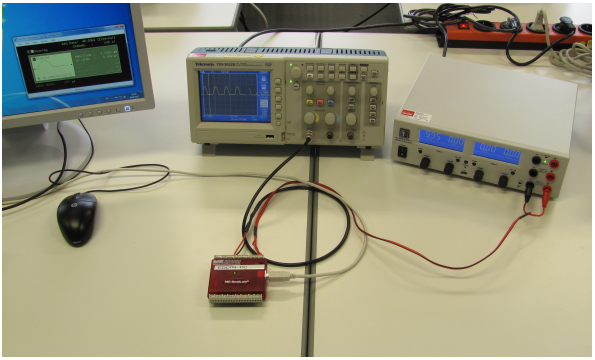
\includegraphics[width=1\textwidth]{../Images/aufbauVersuch1.png}
	\caption{Versuchsaufbau Versuch 1}
\end{figure}
\end{normalsize}

\section{Messwerte}
\label{chap:VERSUCH_1_MESSWERTE}
\begin{normalsize}
\begin{figure}[H]
	\centering
	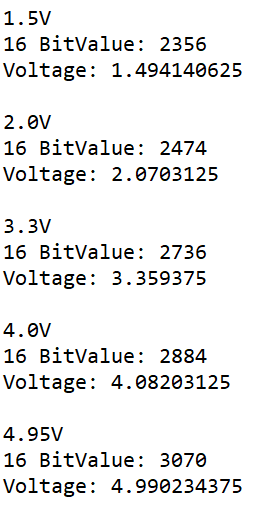
\includegraphics[width=0.3\textwidth]{../Images/messwerteVersuch1.png}
	\caption{Messwerte Versuch 1}
\end{figure}
\end{normalsize}
	
\section{Auswertung}
\label{chap:VERSUCH_1_AUSWERTUNG}
Die eingebene Spannung weicht jedes mal etwas von dem Wert ab, den wir mit dem Feinmessgerät gemessen haben.

\section{Interpretation}
\label{chap:VERSUCH_1_INTERPRETATION}
Der Grund für die Abweichungen könnte thermisches Rauschen sein.
Wir haben zwei Python-Skripte geschrieben, die Konsoleneingaben auf die Karte schreiben können und Daten aus der Karte auslesen könnne. Die Werte haben wir mit einem Messgerät überprüft.
Die Python-Skripte sind im Anhang zu finden.

%
% CHAPTER Versuch 2
%
\chapter{Versuch 2}
\label{chap:VERSUCH_2}

\section{Fragestellung, Messprinzip, Aufbau, Messmittel}
\label{chap:VERSUCH_2_FRAGESTELLUNG}
\begin{normalsize}
Im Zweiten Versuch messen wir Spannungen einer Gleichspannungsquelle von 1V - 10V in 1V Schritten. Diese ermitteln wir mit 3 verschiedenen Messgeräten: einem Multimeter, einem hochgenauen Feinmessgerät und dem AD-Wandler.
Desweiteren sollen wir für das Multimeter und den AD-Wandler die Messfehler und die Standardabweichungen berechnen. Außerdem sollen wir noch den theoretischen Quantisierungsfehler des AD-Wandlers berechnen. Hierfür kamen folgende Dinge zum Einsatz: Python, ME-RedLab USB-1208LS (RedLab-Box), Keithley TRMS 179, Multimeter Philips PM 2503
\begin{figure}[H]
	\centering
	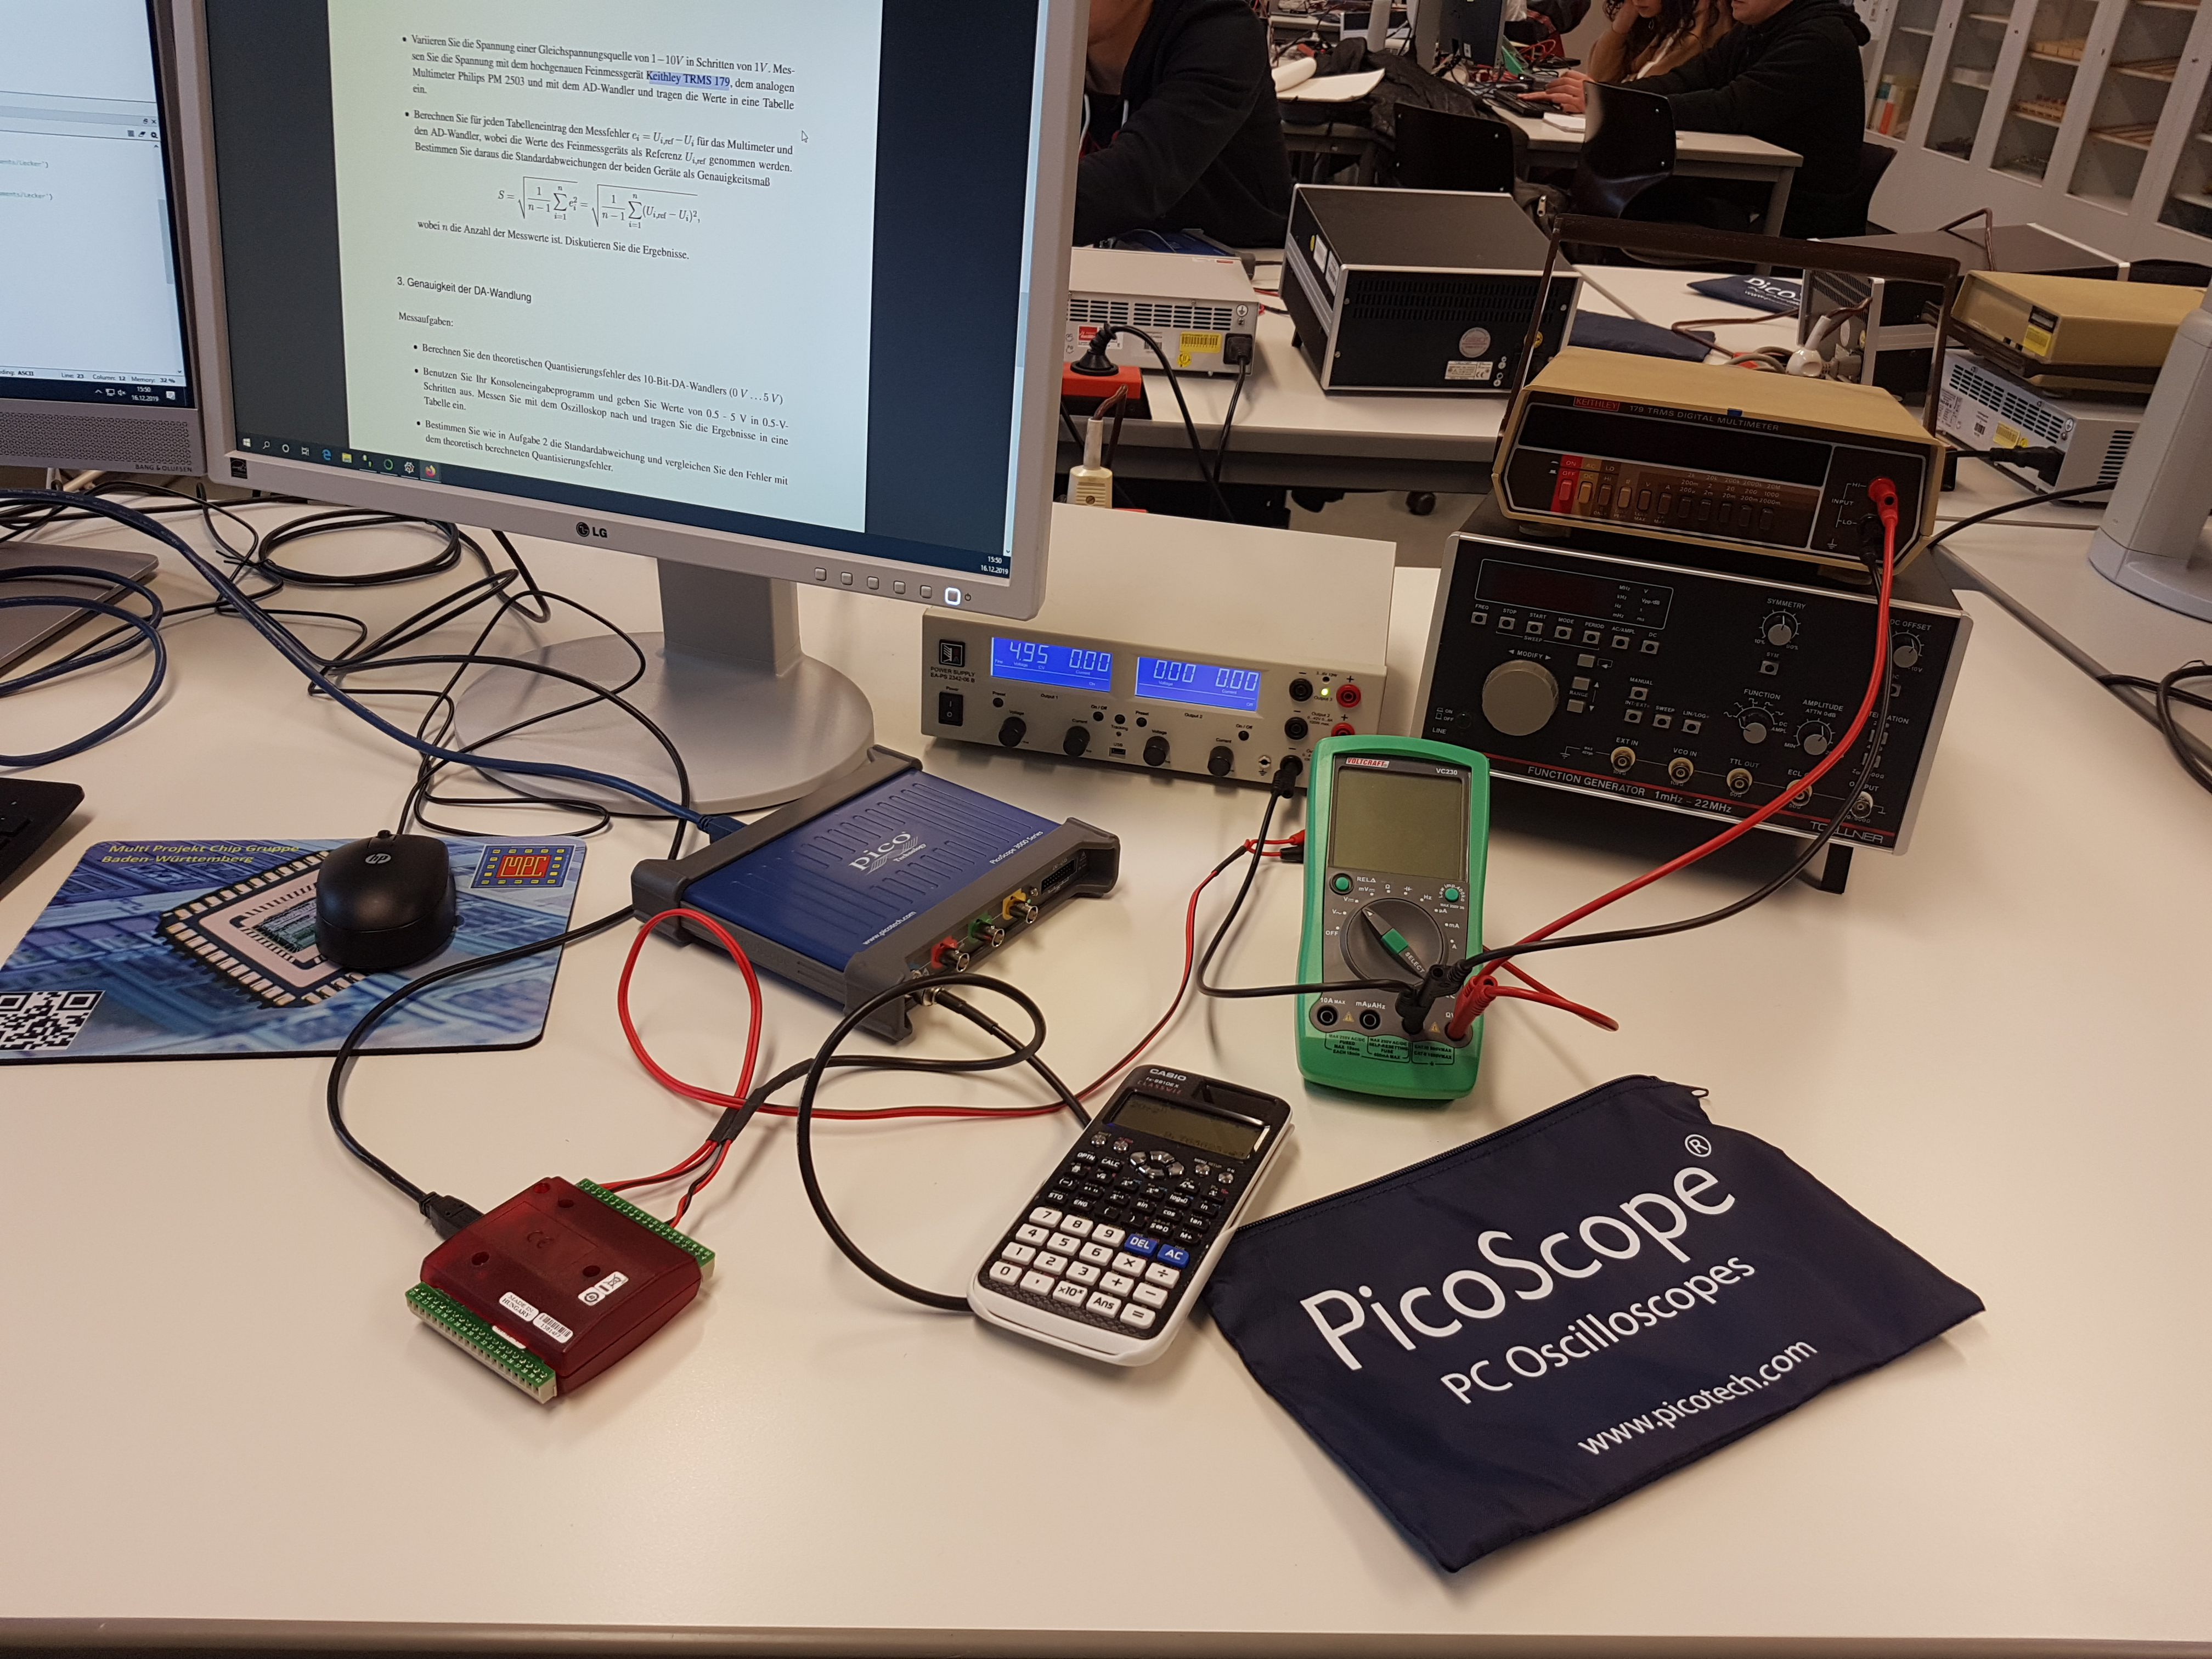
\includegraphics[width=0.7\textwidth]{../Images/aufbauVersuch2.jpg}
	\caption{Versuchsaufbau Versuch 2}
\end{figure}
\end{normalsize}

\section{Messwerte}
\label{chap:VERSUCH_2_MESSWERTE}
\begin{normalsize}
\begin{figure}[H]
	\centering
	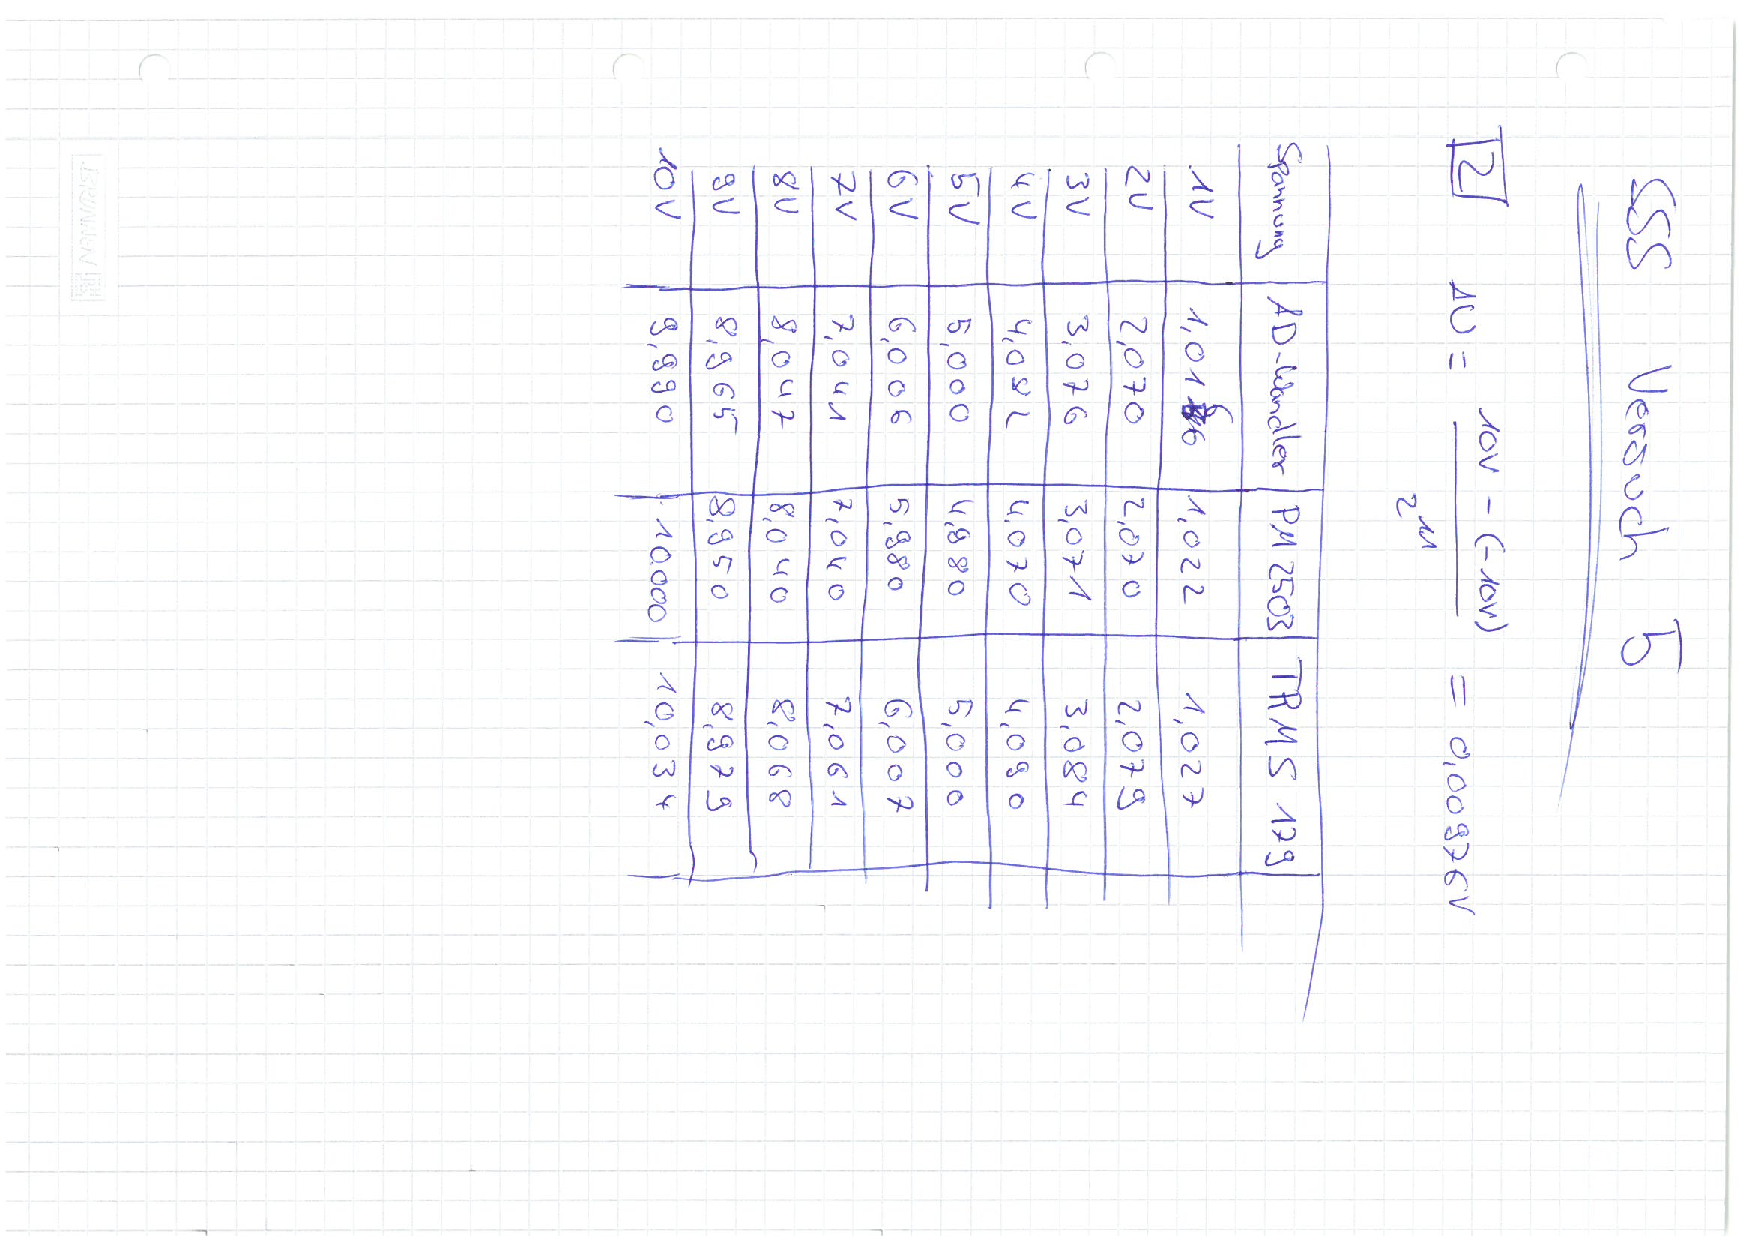
\includegraphics[angle=90,width=0.9\textwidth]{../Messdaten2.pdf}
	\caption{Messwerte Versuch 2}
\end{figure}
\end{normalsize}

\section{Auswertung}
\label{chap:VERSUCH_2_AUSWERTUNG}
\begin{normalsize}
Berechnungen für den Quantisierungsfehler des AD-Wandlers:\newline
\begin{center}
	\begin{tabular}{ l l }
	\textbf{Genauigkeit:} & $\frac{1} {2^n}$ \\
	\textbf{Theoretischer Quantisierungsfehler:} & $\Delta U = \frac{U_{max}  -  U_{min}} {2^n}$ \\
	\end{tabular}
\end{center}
Anzahl Bit des AD-Wandlers = 11\newline
$U_{min}$ = -10 V\newline
$U_{max}$ = 10 V\newline
Theoretischer Quantisierungsfehler des AD-Wandlers = 0,00976 V\newline\newline
Berechnungen für die Messfehler und die Standardabweichungen der Geräte:\newline
\begin{center}
	\begin{tabular}{ l l }
	\textbf{Messfehler:} & $e_i = U_{i,ref} - U_i$ \\
	\textbf{Standardabweichung:} & $S = \sqrt{\frac{1} {n - 1} \sum_{i = 1}^n e_i^2 }$ \\
	\end{tabular}
\end{center}
\centering
\begin{tabular}{*{3}{c|c|c|p{2cm}}}
Feinmessgerät (V) & Messfehler Multimeter (V) & Messfehler AD-Wandler (V) \\
\hline
1,027 & 0,005 & 0,011 \\
2,079 & 0,009 & 0,009 \\
3,084 & 0,013 & 0,008 \\
4,090 & 0,020 & 0,008 \\
5,000 & 0,020 & 0,000 \\
6,007 & 0,027 & 0,001 \\
7,061 & 0,021 & 0,020 \\
8,068 & 0,028 & 0,021 \\
8,979 & 0,029 & 0,014 \\
10,034 & 0,034 & 0,044 \\

\end{tabular}
\captionof{table}{Messwerte und Messfehler}
Standardabweichung Multimeter: S = 0,0229\newline
Standardabweichung AD-Wandler: S = 0,0147\newline
\end{normalsize}

\section{Interpretation}
\label{chap:VERSUCH_2_INTERPRETATION}
\begin{normalsize}
Man kann sehen, dass das Feinmessgerät auch nicht ganz genau ist. Die Messfehler der beiden anderen Messgeräte unterscheiden sich ziemlich. Der AD-Wandler hat im Schnitt deutlich geringere Messfehler, als das Multimeter.
Dies sieht man auch an der Standardabweichung, die beim AD-Wandler viel kleiner ist. Die Standardabweichung des AD-Wandlers entspricht ungefähr dem theoretischen Quantisierungsfehler.
\end{normalsize}

%
% CHAPTER Versuch 3
%
\chapter{Versuch 3}
\label{chap:VERSUCH_3}

\section{Fragestellung, Messprinzip, Aufbau, Messmittel}
\label{chap:VERSUCH_3_FRAGESTELLUNG}
\begin{normalsize}
Im 3. Versuch untersuchen wir die Genauigkeit des 10-Bit-DA-Wandlers (0 V ... 5 V). Dafür berechnen wir zunächst den theoretischen Quantisierungsfehler. Anschließend geben wir Werte von 0.5 V - 5V in 0.5 V Schritten aus und
messen diese mit dem Oszilloskop nach. Zum Schluss bestimmen wir, wie im 2. Versuch, die Standardabweichung und vergleichen diese mit dem Quantisierungsfehler. Der Versuchsaufbau ist wie beim 1. Versuch. Es kamen folgende Dinge zum Einsatz: Python, ME-RedLab USB-1208LS (RedLab-Box), Oszilloskop.
\end{normalsize}

\section{Messwerte}
\label{chap:VERSUCH_3_MESSWERTE}
\begin{normalsize}
\begin{figure}[H]
	\centering
	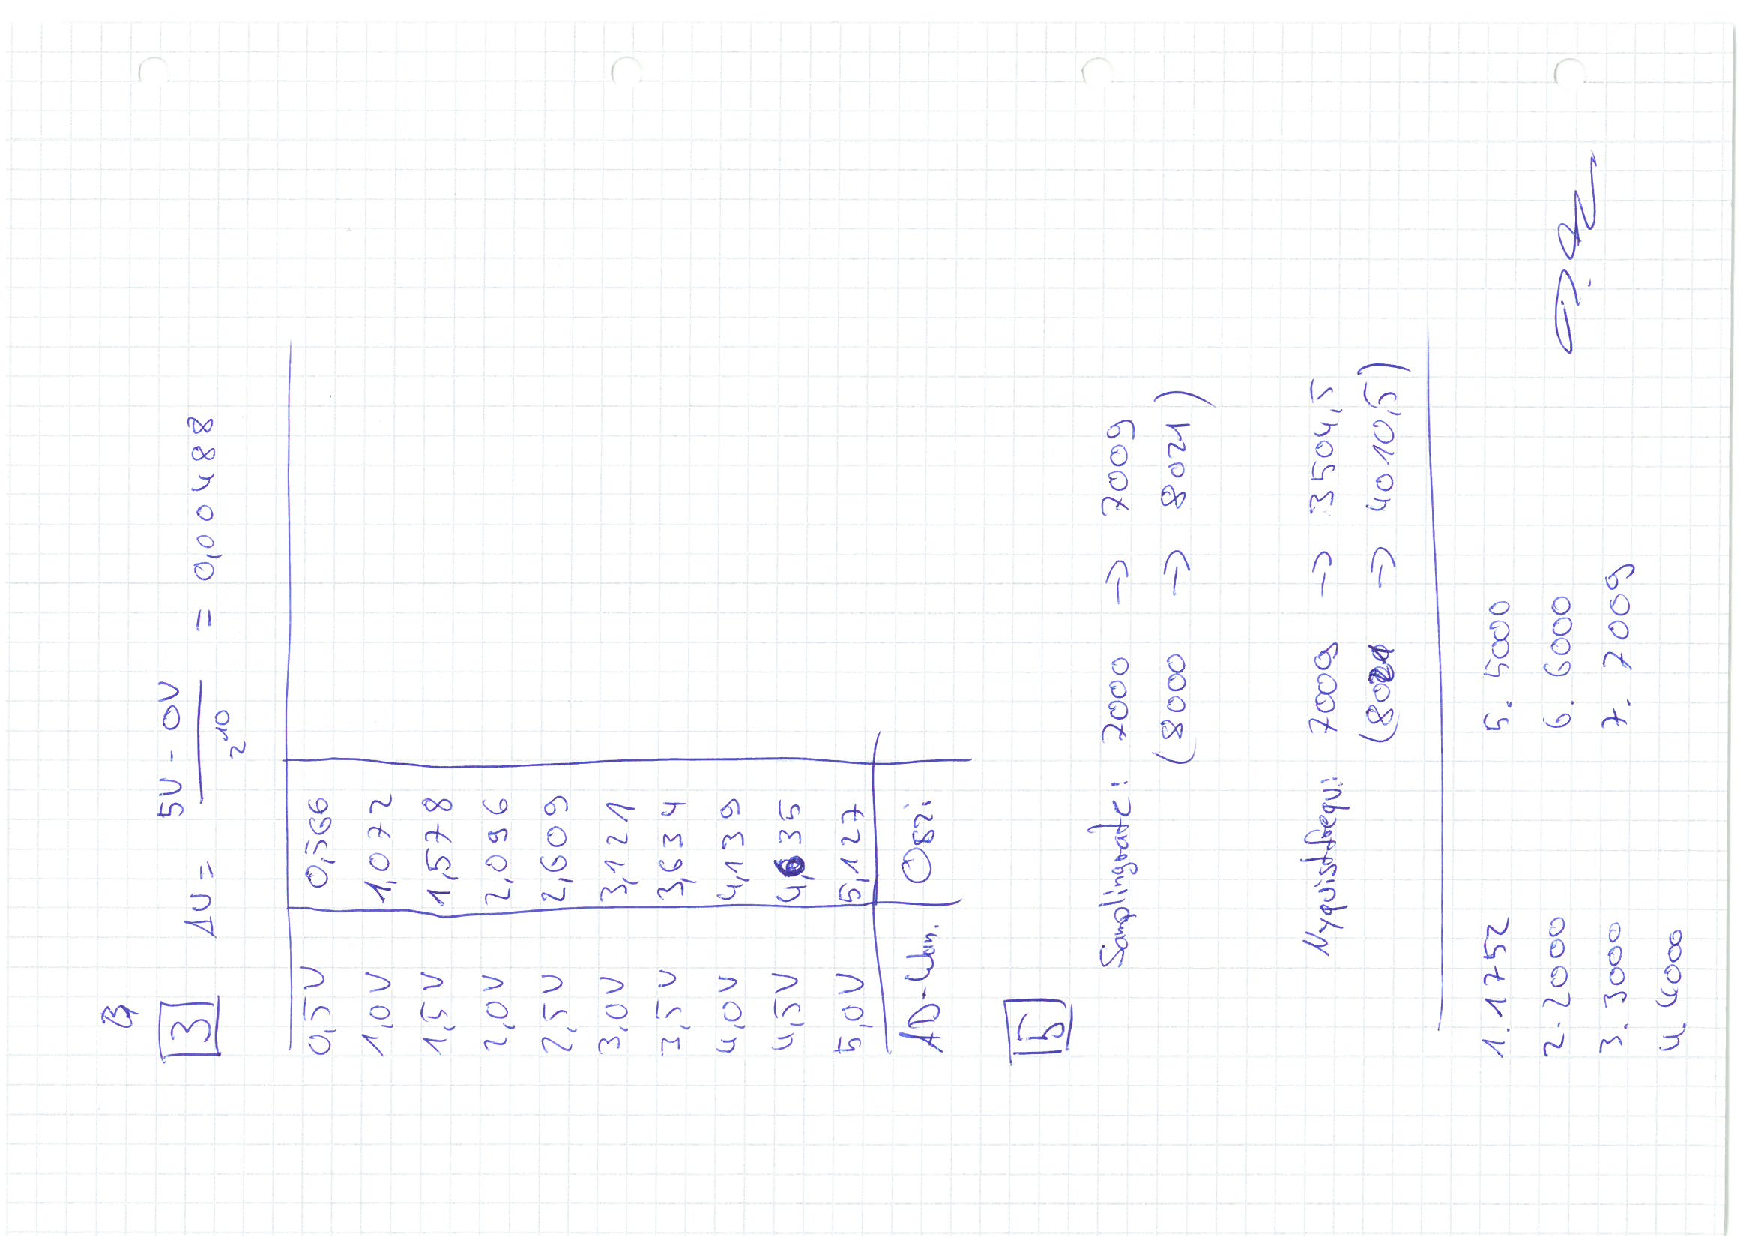
\includegraphics[angle=270,width=0.9\textwidth]{../Messdaten3.pdf}
	\caption{Messwerte Versuch 3}
\end{figure}
\end{normalsize}

\section{Auswertung}
\label{chap:VERSUCH_3_AUSWERTUNG}
\begin{normalsize}
Berechnungen für den Quantisierungsfehler des DA-Wandlers:\newline
\begin{center}
	\begin{tabular}{ l l }
	\textbf{Genauigkeit:} & $\frac{1} {2^n}$ \\
	\textbf{Theoretischer Quantisierungsfehler:} & $\Delta U = \frac{U_{max}  -  U_{min}} {2^n}$ \\
	\end{tabular}
\end{center}
Anzahl Bit des DA-Wandlers = 10\newline
$U_{min}$ = 0 V\newline
$U_{max}$ = 5 V\newline
Theoretischer Quantisierungsfehler des DA-Wandlers = 0,00488 V\newline\newline
Berechnungen für die Messfehler und die Standardabweichung des DA-Wandlers:\newline
\begin{center}
	\begin{tabular}{ l l }
	\textbf{Messfehler:} & $e_i = U_{i,ref} - U_i$ \\
	\textbf{Standardabweichung:} & $S = \sqrt{\frac{1} {n - 1} \sum_{i = 1}^n e_i^2 }$ \\
	\end{tabular}
\end{center}
\centering
\begin{tabular}{*{3}{c|c|c|p{2cm}}}
Referenzwerte (V) & Oszilloskop (V) & Messfehler DA-Wandler (V) \\
\hline
0,5 & 0,566 & 0,066 \\
1,0 & 1,072 & 0,072 \\
1,5 & 1,578 & 0,078 \\
2,0 & 2,096 & 0,096 \\
2,5 & 2,609 & 0,109 \\
3,0 & 3,121 & 0,121 \\
3,5 & 3,634 & 0,134 \\
4,0 & 4,139 & 0,139 \\
4,5 & 4,635 & 0,135 \\
5,0 & 5,127 & 0,127 \\

\end{tabular}
\captionof{table}{Messwerte und Messfehler}
Standardabweichung des DA-Wandlers: S = 0,1197\newline
\end{normalsize}

\pagebreak

\section{Interpretation}
\label{chap:VERSUCH_3_INTERPRETATION}
\begin{normalsize}
Aus der Tabelle kann man ablesen, dass der Messfehler größer wird, wenn auch die Spannung größer wird. Die Standardabweichung des DA-Wandlers ist deutlich größer als der theoretische Quantisierungsfehler. Außerdem ist die Standardabweichung auch größer, als die des AD-Wandlers, nämlich ungefähr um den Faktor 10.
Daraus lässt sich schließen, dass die Wandlung eines digitalen Signals in ein Analoges viel fehlerbehafteter ist, als andersherum. Dies könnte zum Beispiel an thermischem Rauschen oder an Rundungsfehlern liegen. 
\end{normalsize}

%
% CHAPTER Versuch 4
%
\chapter{Versuch 4}
\label{chap:VERSUCH_4}

\section{Fragestellung, Messprinzip, Aufbau, Messmittel}
\label{chap:VERSUCH_4_FRAGESTELLUNG}
\begin{normalsize}
Die Aufgabe im vorletzten Teil des letzen Versuches ist es ein Programm zu schreiben, welches eine Sinusspannung ausgibt.
Dazu sollen die Werte sequentiell hintereinander auf die Karte geschrieben werden,
wobei zwischen den einzelnen Ausgaben geeignete Pausen eingehalten werden müssen um die Samplingrate des DA-Wandlers einzuhalten.	
\end{normalsize}

\section{Messwerte}
\label{chap:VERSUCH_4_MESSWERTE}
Hier ist der ausgegebene Spannungsverlauf auf dem Oszilloskop zu sehen:
\begin{figure}[H]
	\centering
	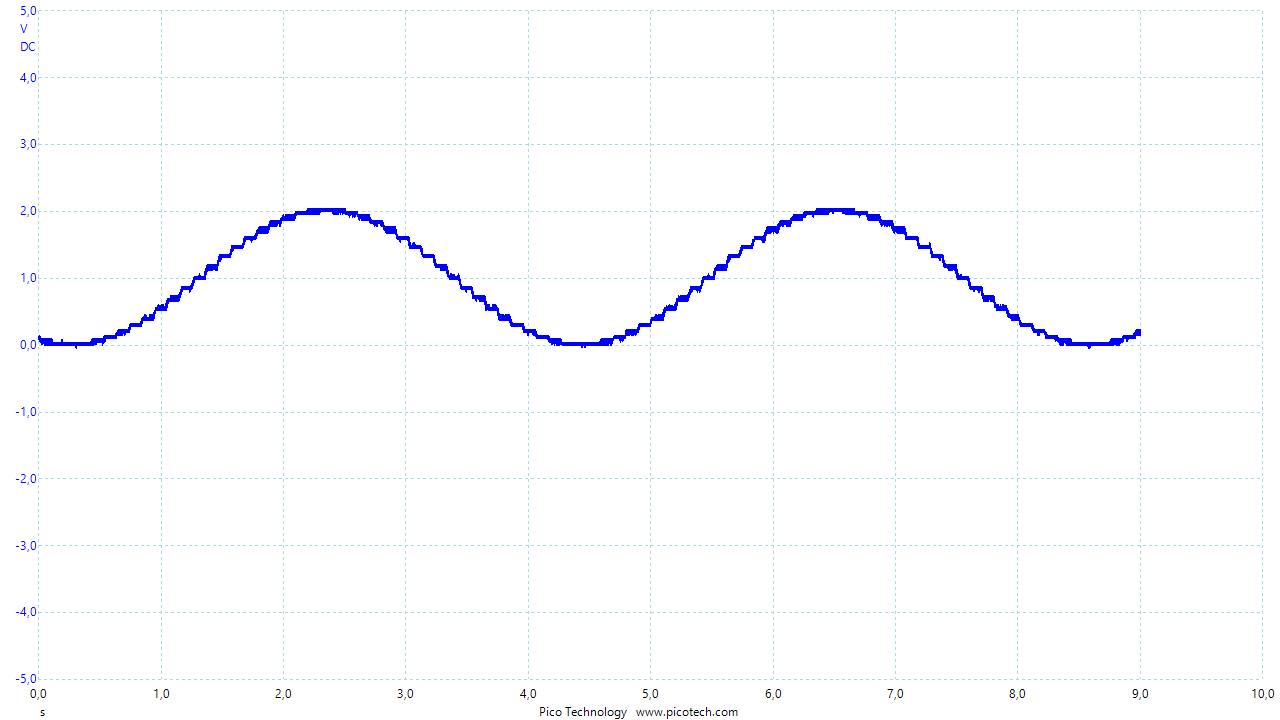
\includegraphics[width=0.8\textwidth]{../Images/Sinus.png}
	\caption{Sinus}
\end{figure}

\section{Auswertung}
\label{chap:VERSUCH_4_AUSWERTUNG}
\begin{normalsize}
In der oben stehenden Abbildung ist gut zu sehen, dass es sich hier um einen
Sinus handelt der um 1 nach oben verschoben wurde. Auserderm ist sehr gut zu erkennen,
dass die Linie nicht kontinuirlich verläuft sondern aus Treppenstufen besteht.
\end{normalsize}

\section{Interpretation}
\label{chap:VERSUCH_4_INTERPRETATION}
\begin{normalsize}
Die in der Abbildung zu sehenden Treppenstufen ensteht durch die digitale Ausgansspannung des AD-Wandlers.
Der Sinus kann also nur in diskreten Schritten nachgebildet werden. Je höher die Auflösung des Wandlers umso feiner sind
die Stufen im nachgebildeten Sinus. 
\end{normalsize}
%
% CHAPTER Versuch 5
%
\chapter{Versuch 5}
\label{chap:VERSUCH_5}

\section{Fragestellung, Messprinzip, Aufbau, Messmittel}
\label{chap:VERSUCH_5_FRAGESTELLUNG}
\begin{normalsize}
	Im letzten Abschnitt des Versuches wählen wir ein Abtastfrequenz im Intervall von 6000 - 8000 Herz aus.
	Mit Python und dem entsprechenden RedLab-Befehl lesen wir die tatsächliche Abtastfrequenz des AD-Wandlers für unsere gewählte Abtastfrequenz aus.
	\newline
	Anschließend variieren wir, angefangen von der halben Nyquist-Frequenz bis zur doppelten Nyquist-Frequenz,
	die Frequenz des Sinusgenerators in 7 Schritten und plotten die entsprechenden Kurven mit Python.
\end{normalsize}
\newline
\newline
Was ist hier also die Nyquist-Frequenz?
\section{Messwerte}
\label{chap:VERSUCH_5_MESSWERTE}
\begin{figure}[H]
	\centering
	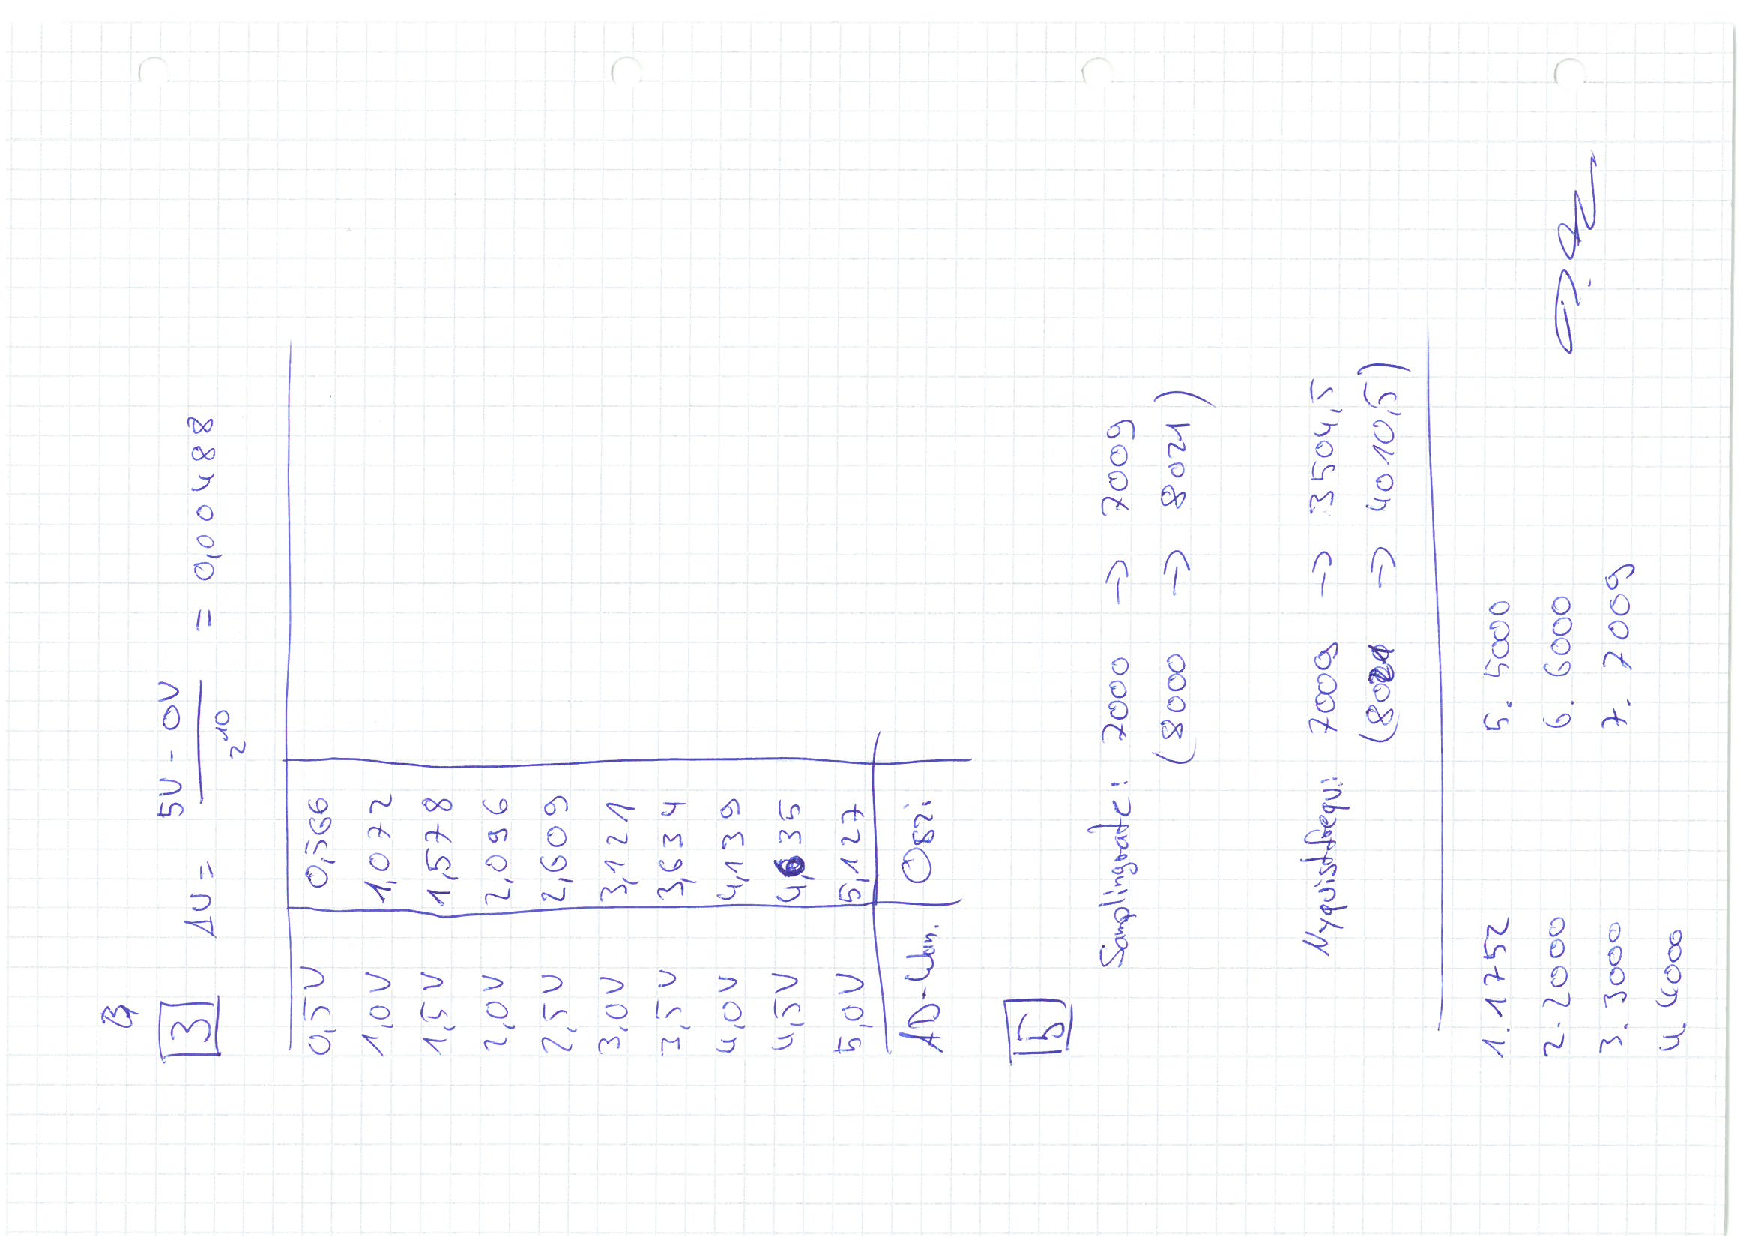
\includegraphics[angle=270,width=0.9\textwidth]{../Messdaten3.pdf}
	\caption{Messwerte Versuch 5}
\end{figure}

\section{Auswertung}
\label{chap:VERSUCH_5_AUSWERTUNG}
\begin{figure}[H]
	\centering
	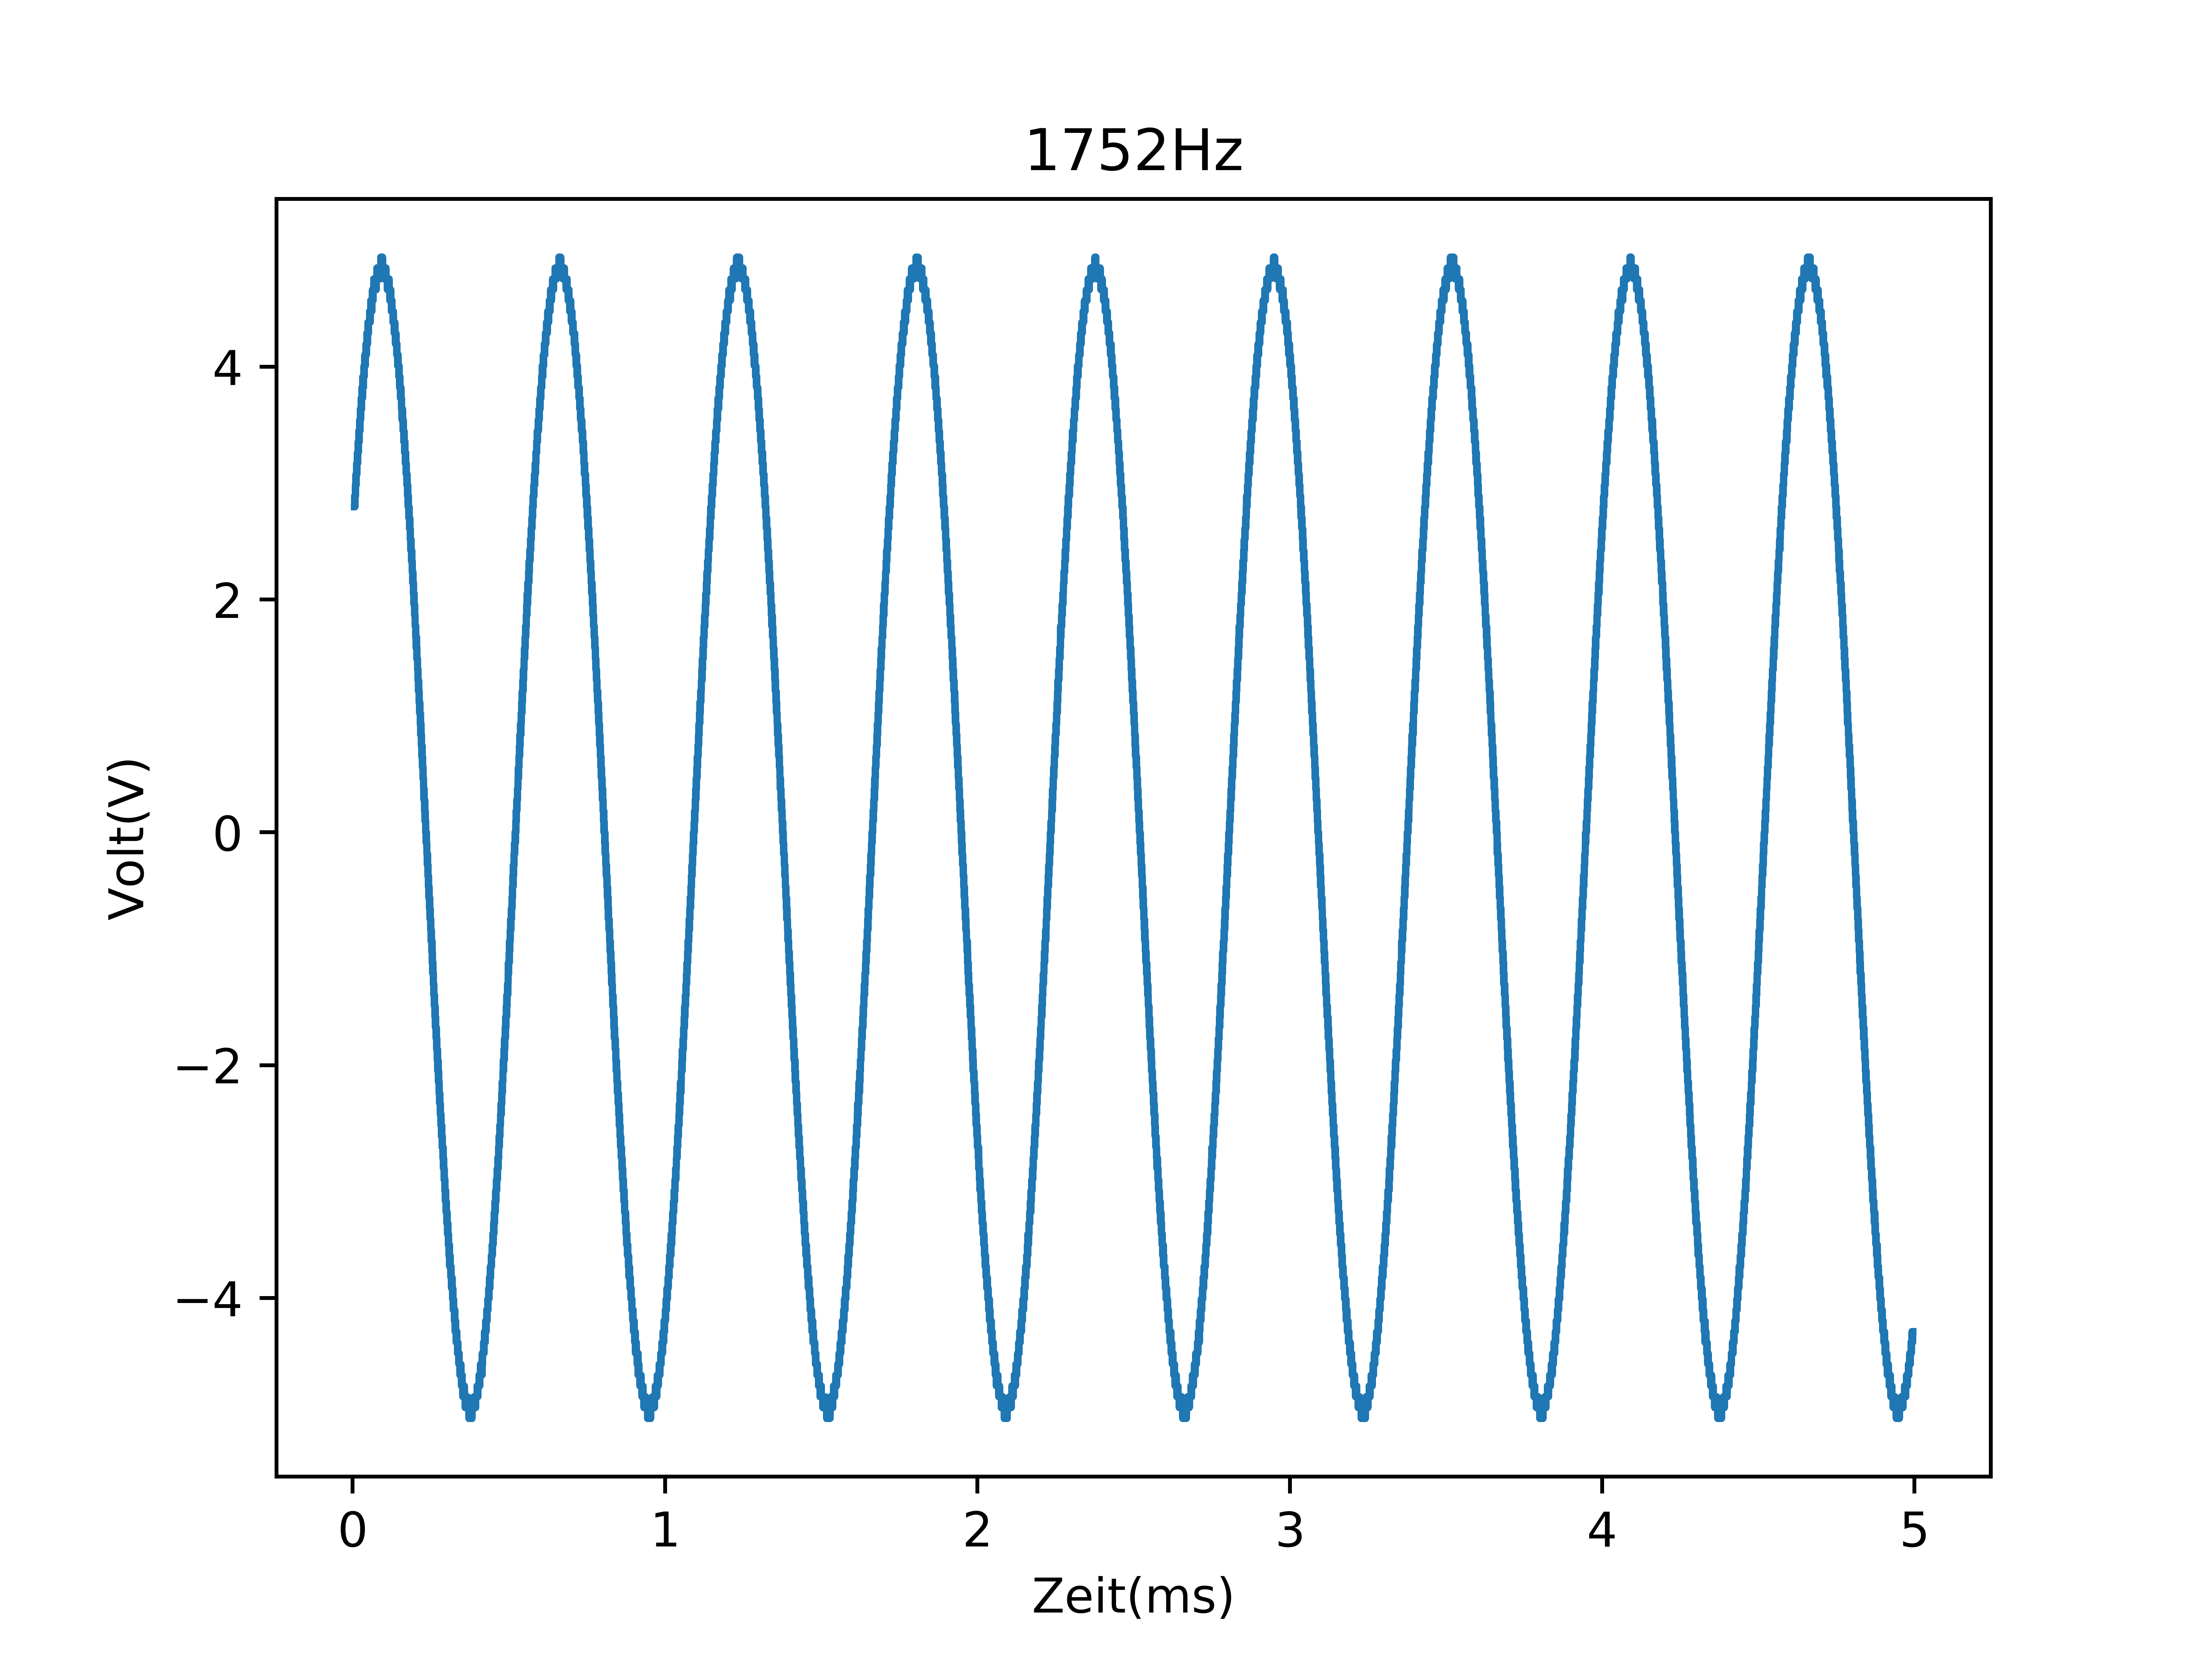
\includegraphics[width=0.8\textwidth]{../Images/1752Hz.png}
	\caption{1752Hz}
\end{figure}
\begin{figure}[H]
	\centering
	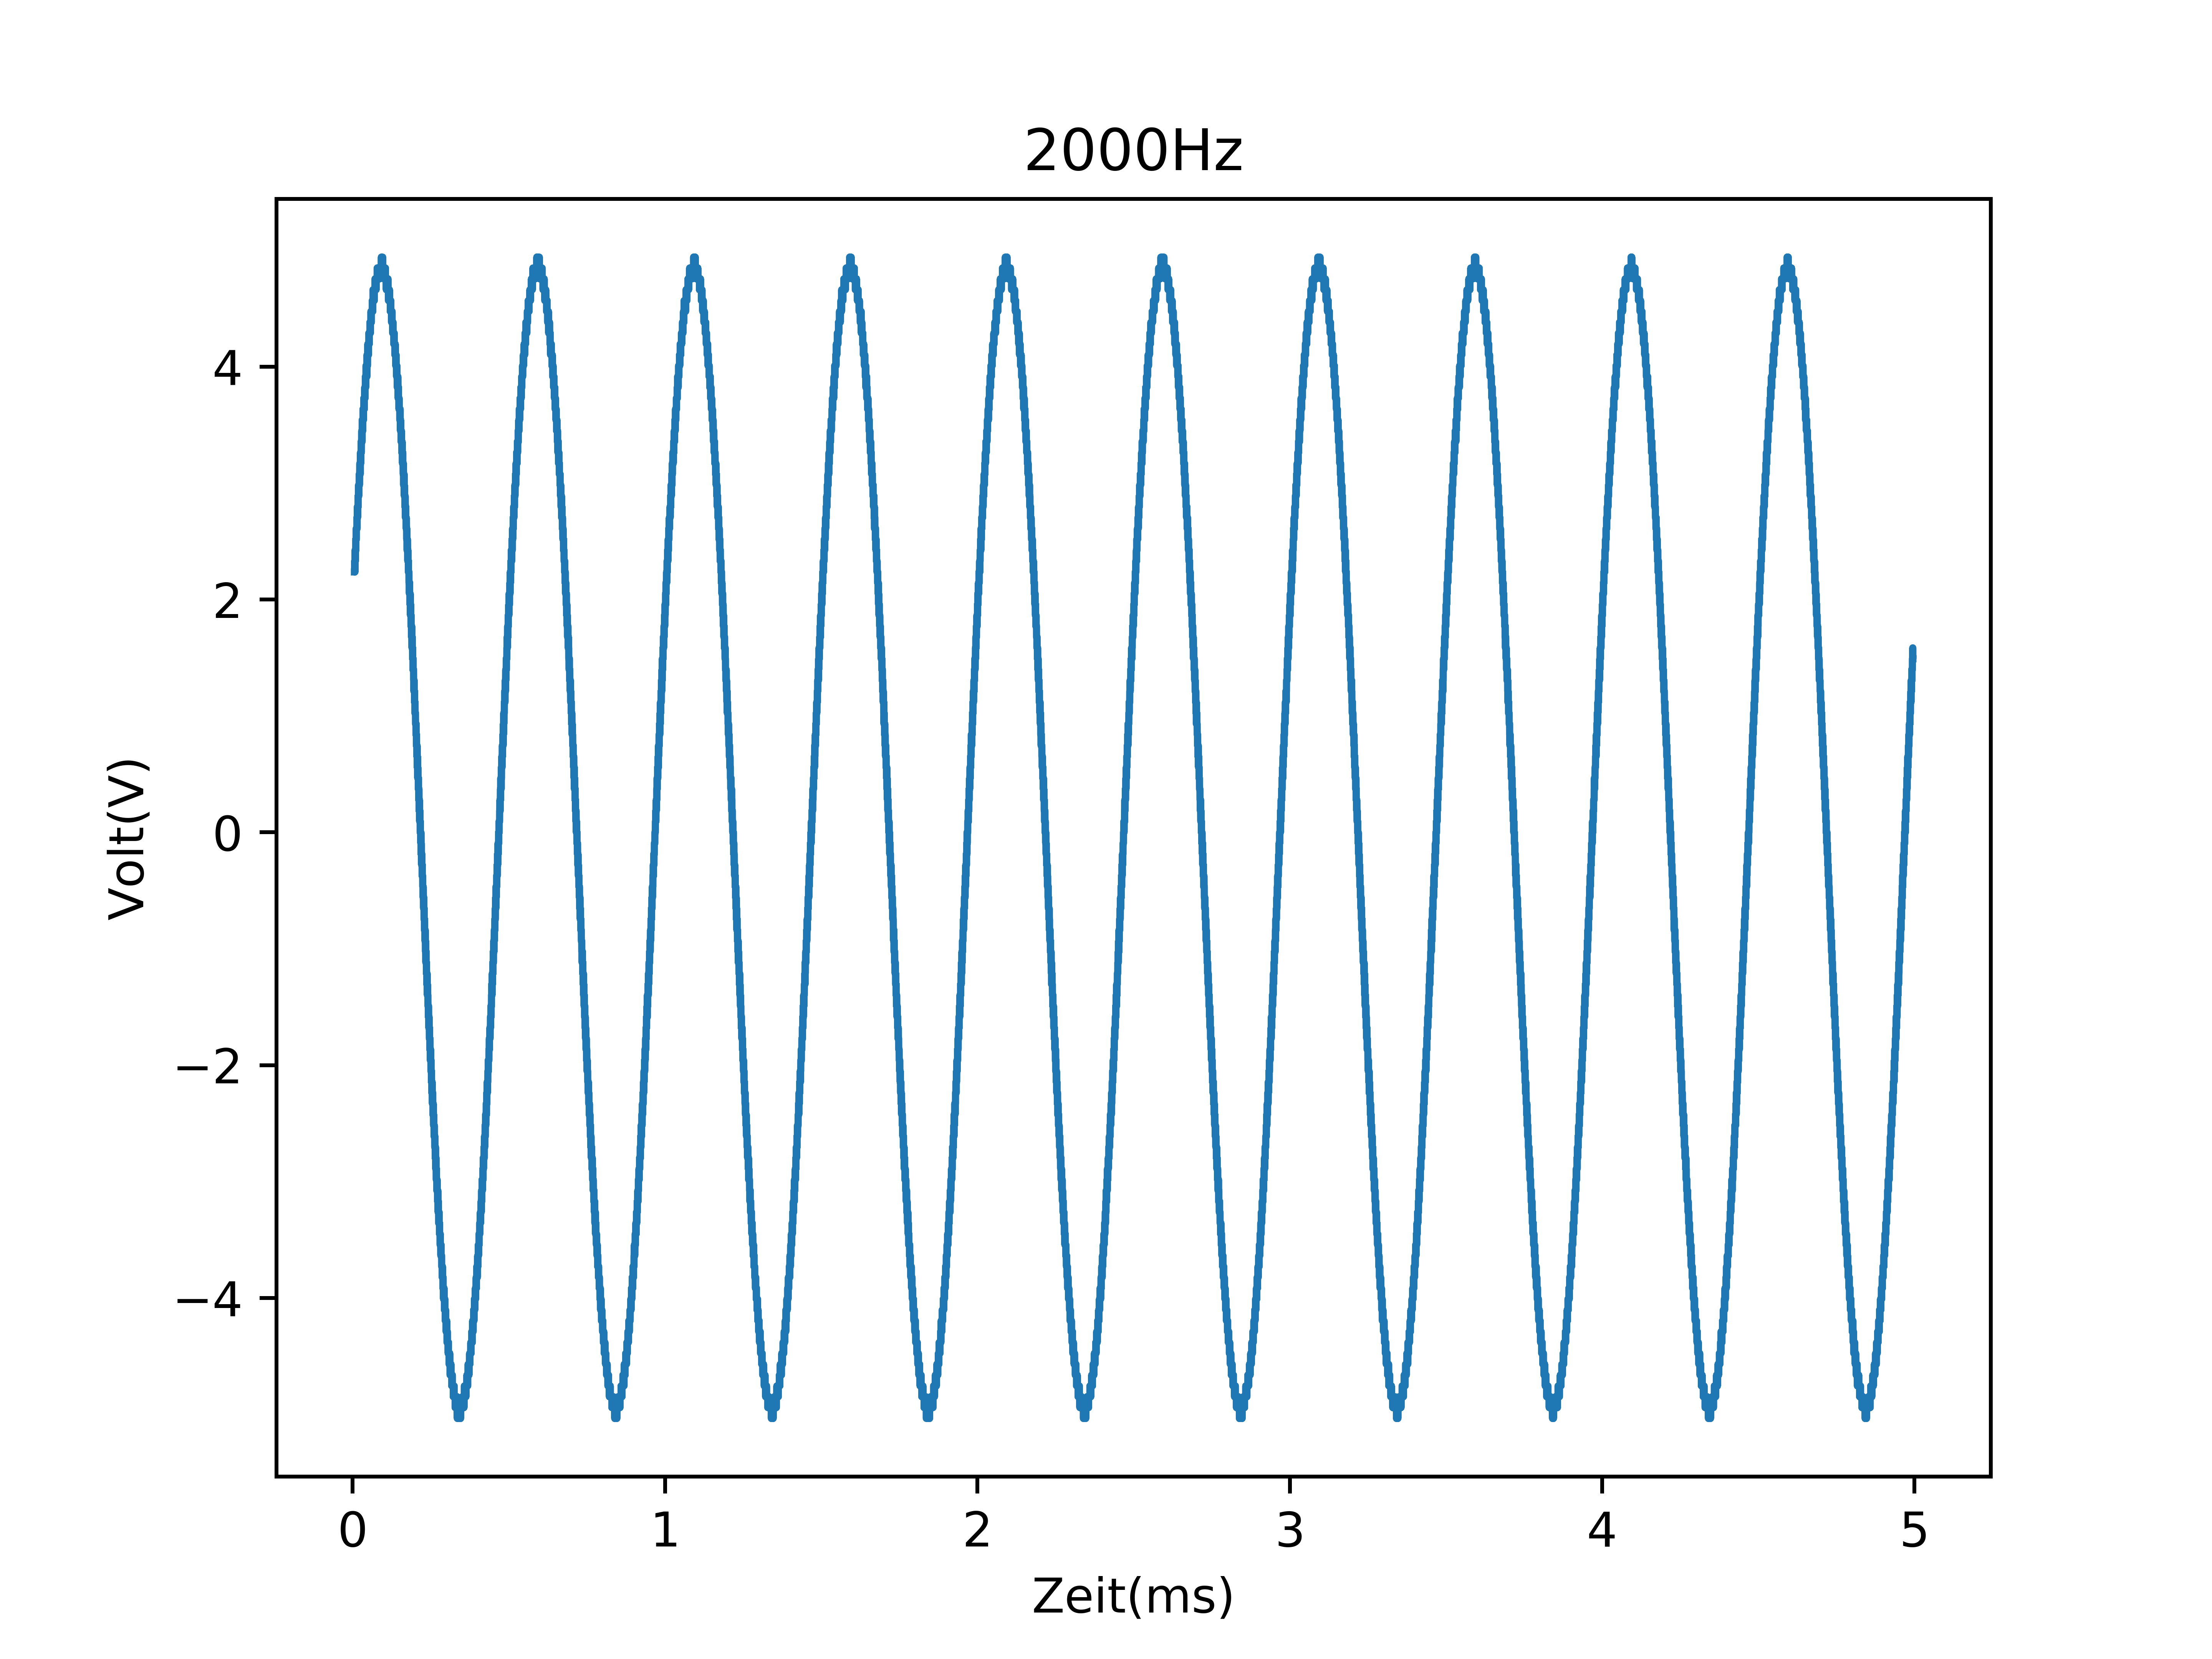
\includegraphics[width=0.8\textwidth]{../Images/2000Hz.png}
	\caption{2000Hz}
\end{figure}
\begin{figure}[H]
	\centering
	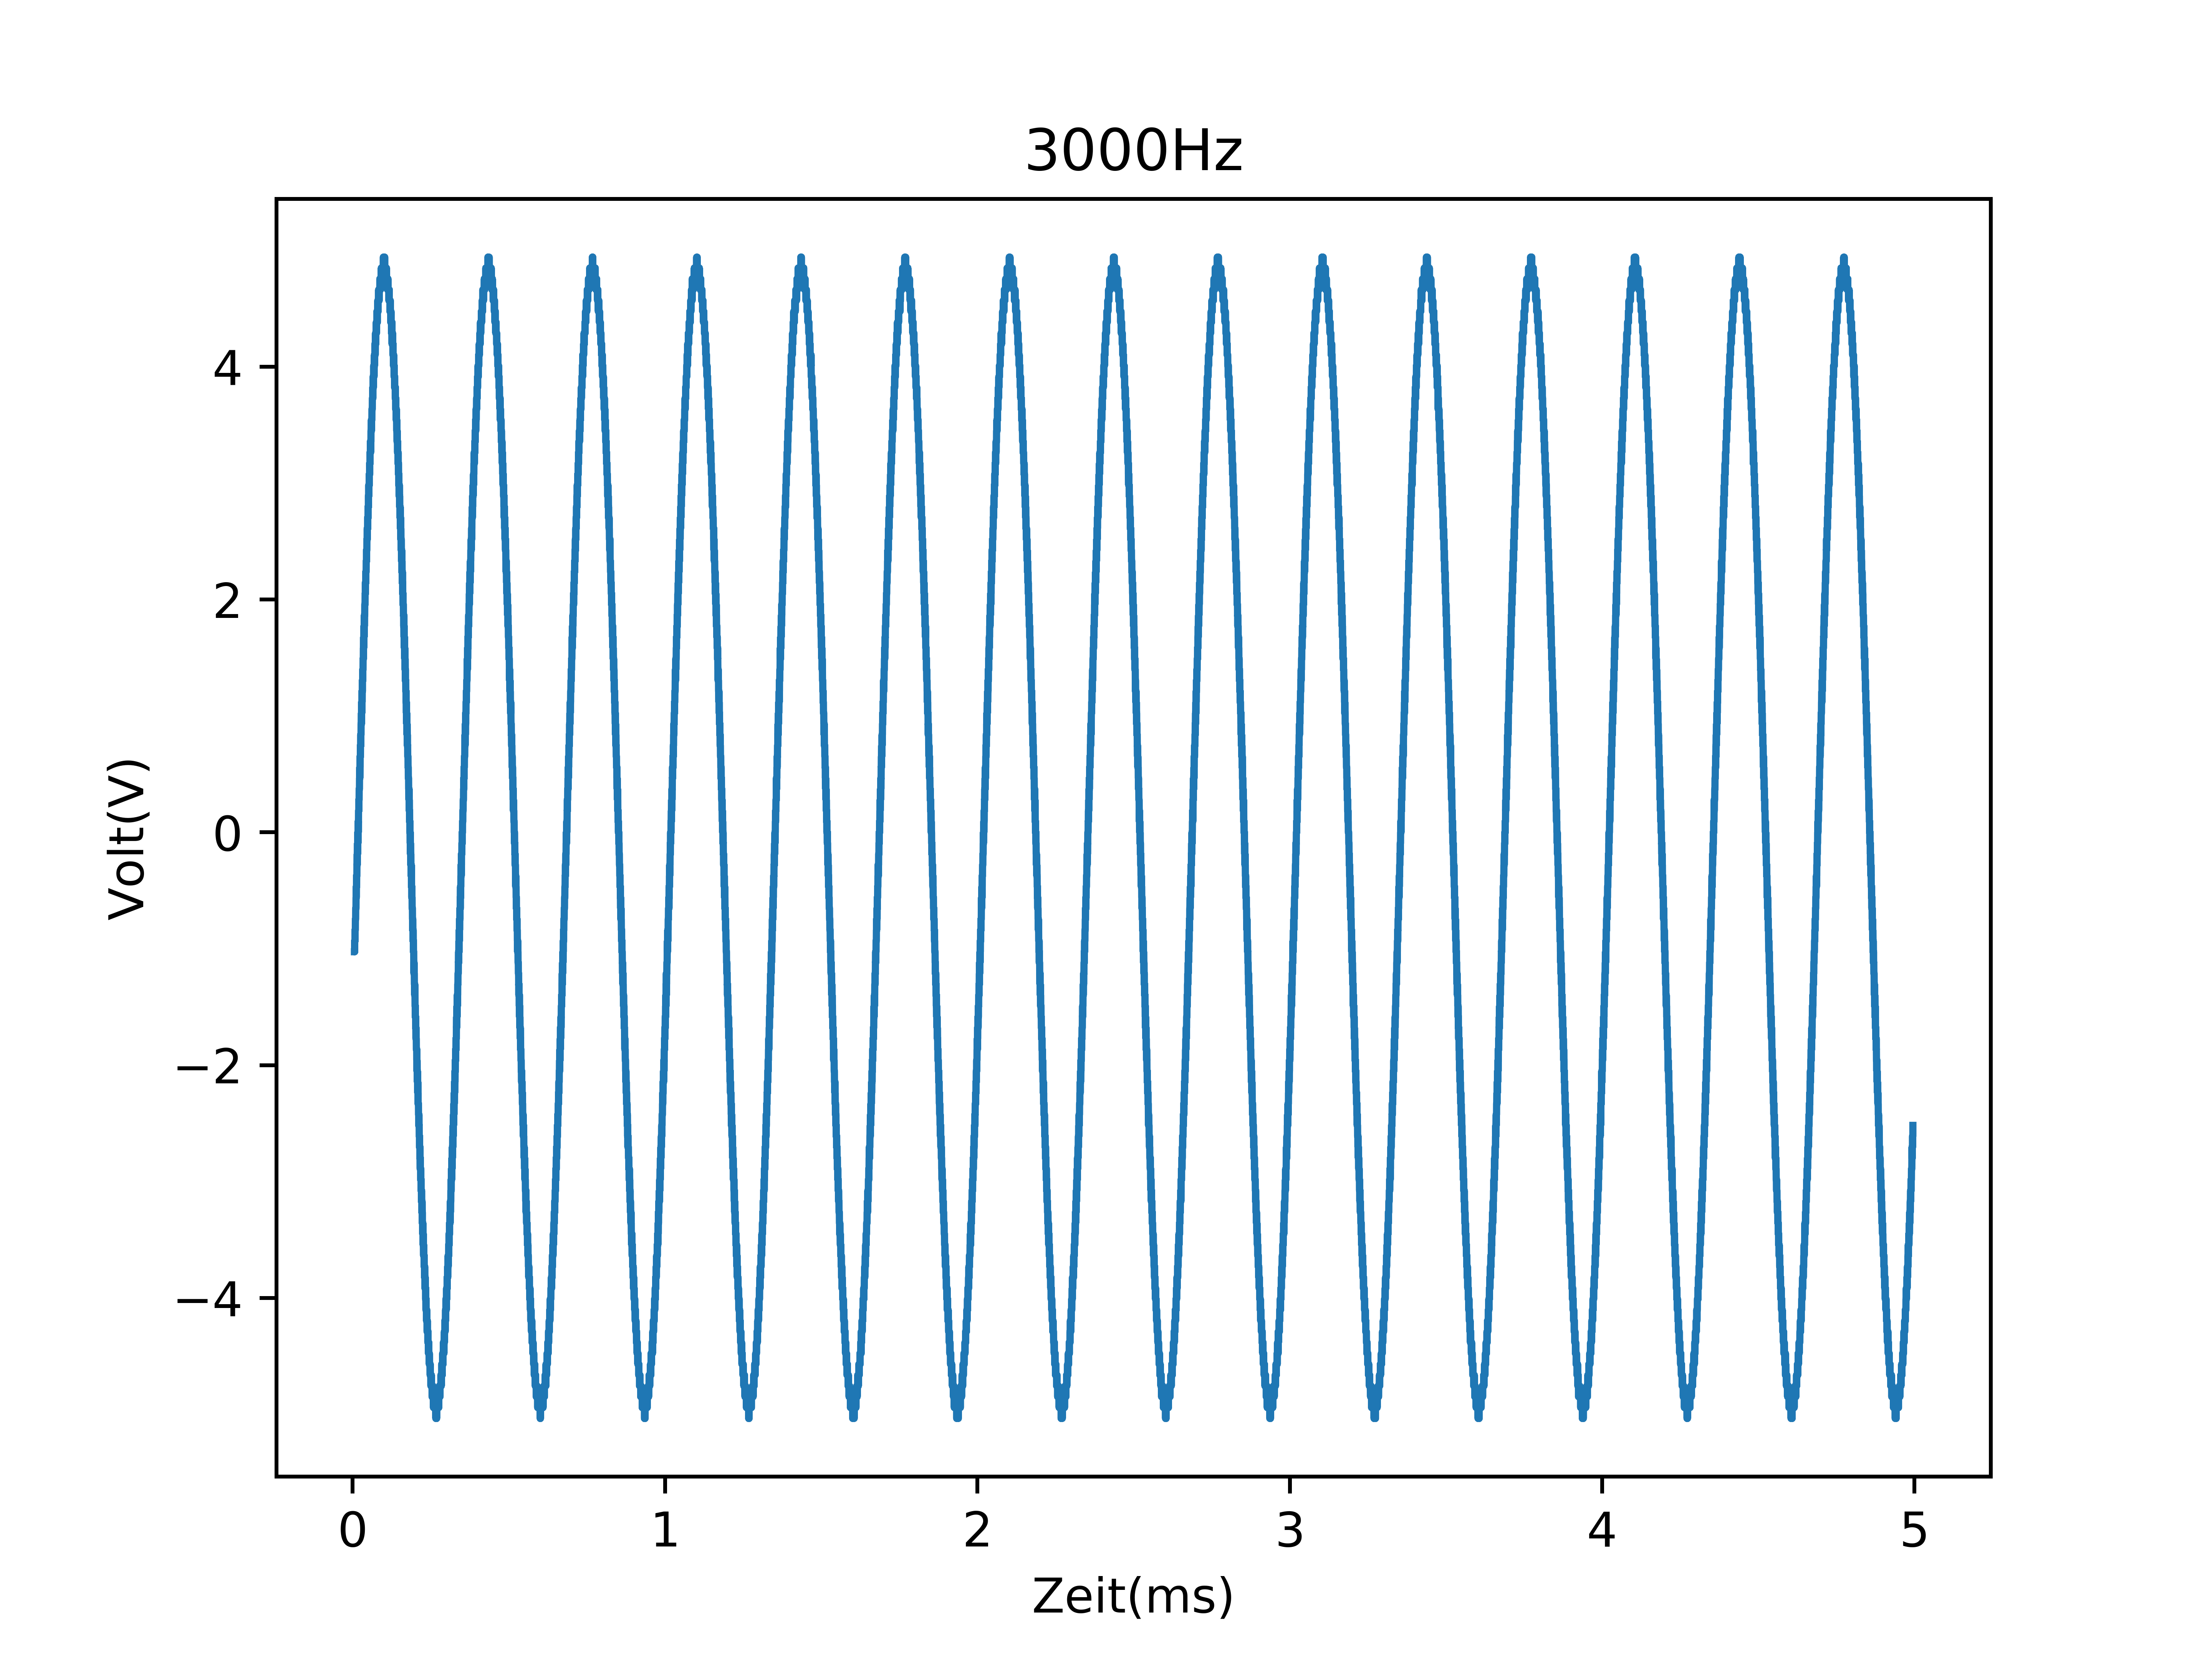
\includegraphics[width=0.8\textwidth]{../Images/3000Hz.png}
	\caption{3000Hz}
\end{figure}
\begin{figure}[H]
	\centering
	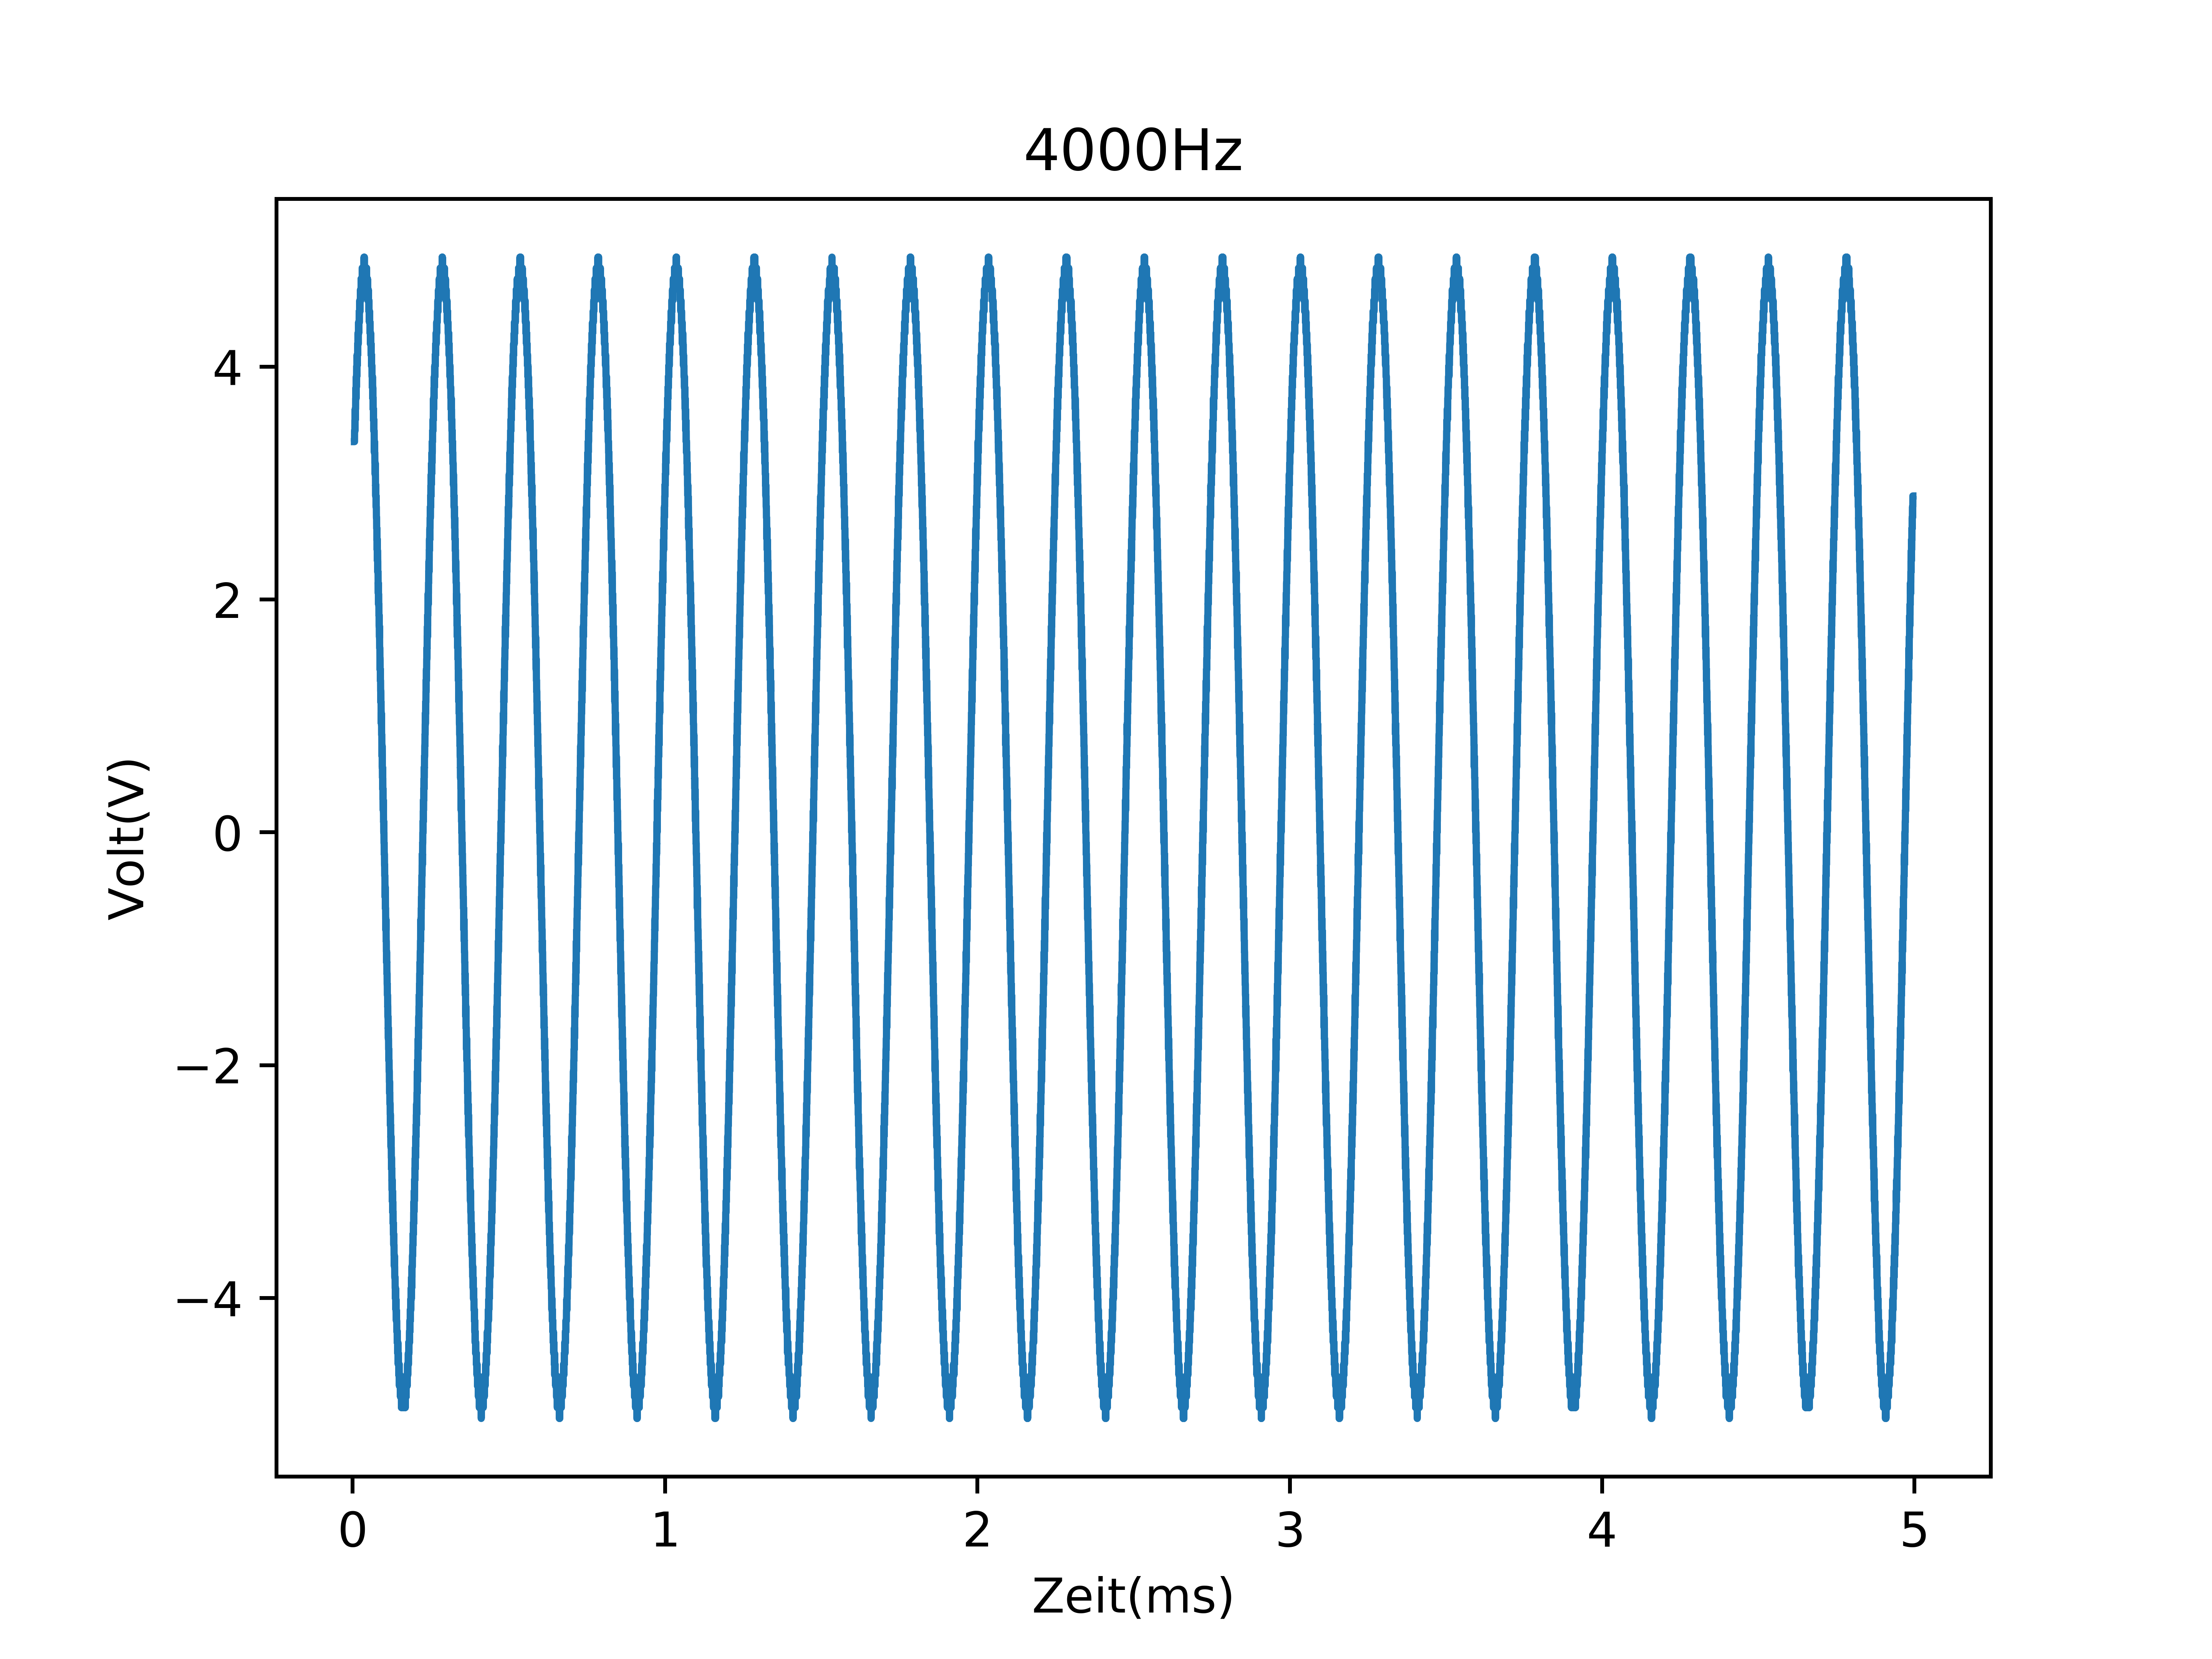
\includegraphics[width=0.8\textwidth]{../Images/4000Hz.png}
	\caption{4000Hz}
\end{figure}
\begin{figure}[H]
	\centering
	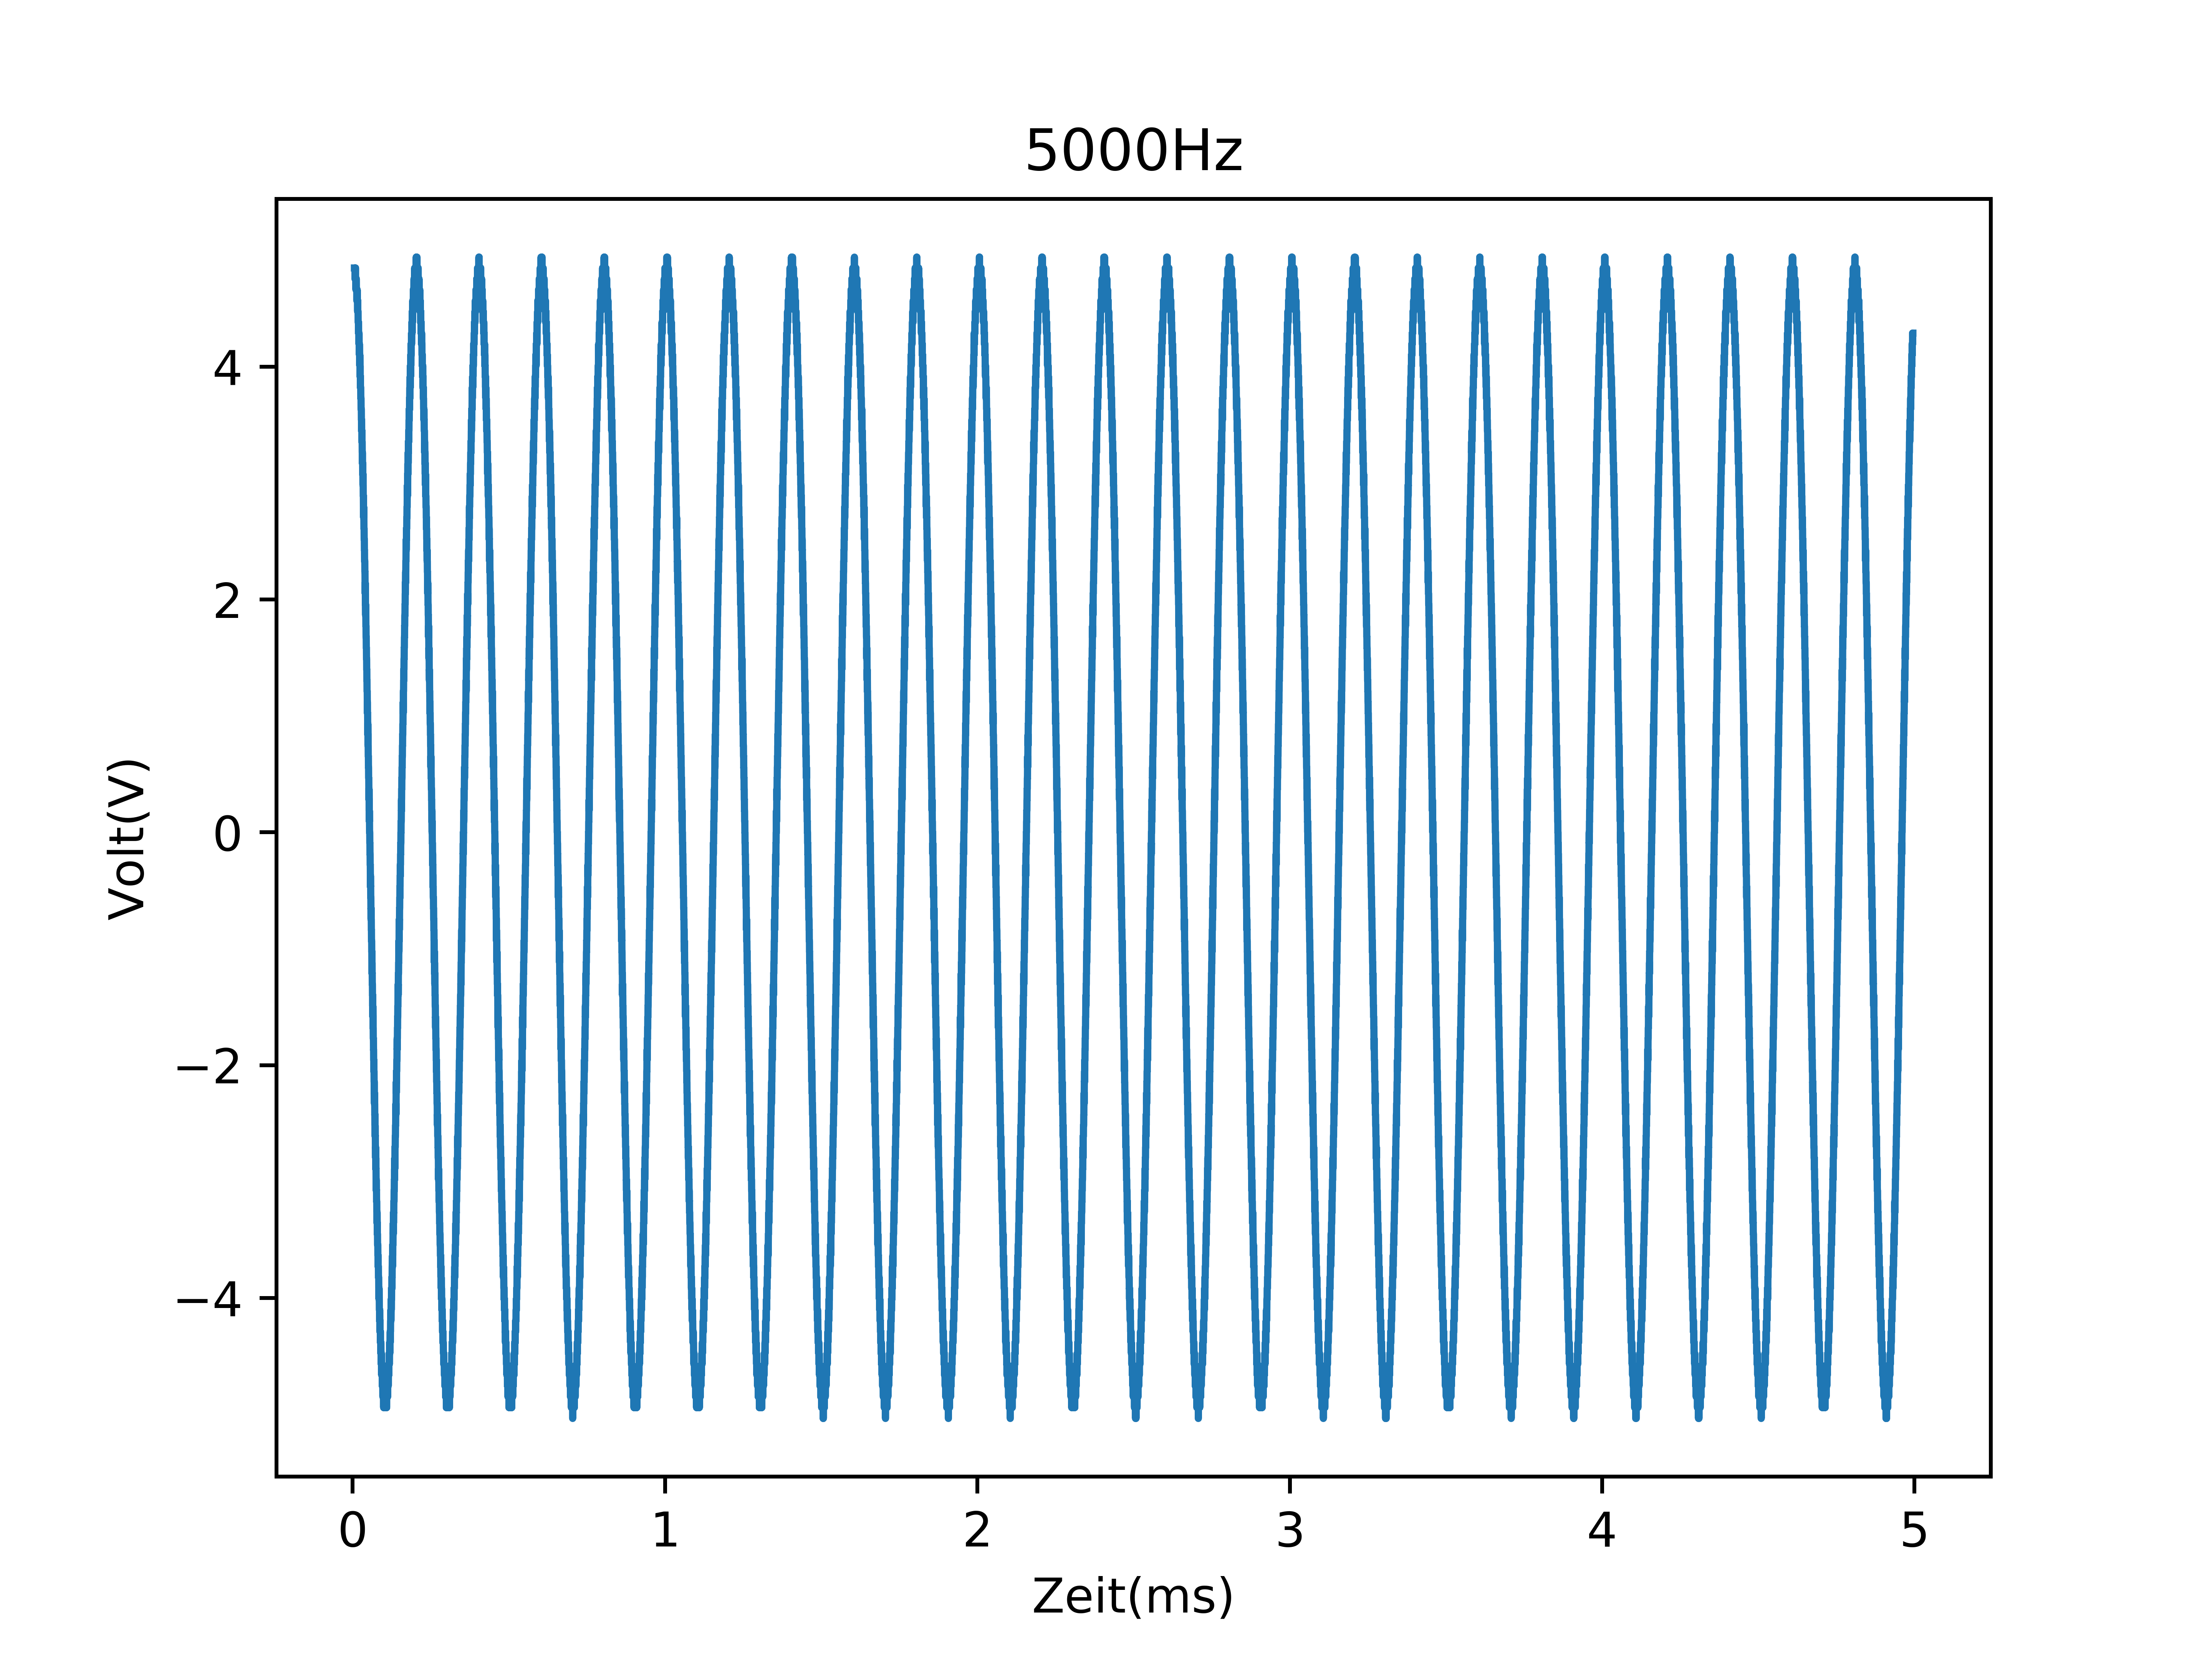
\includegraphics[width=0.8\textwidth]{../Images/5000Hz.png}
	\caption{5000Hz}
\end{figure}
\begin{figure}[H]
	\centering
	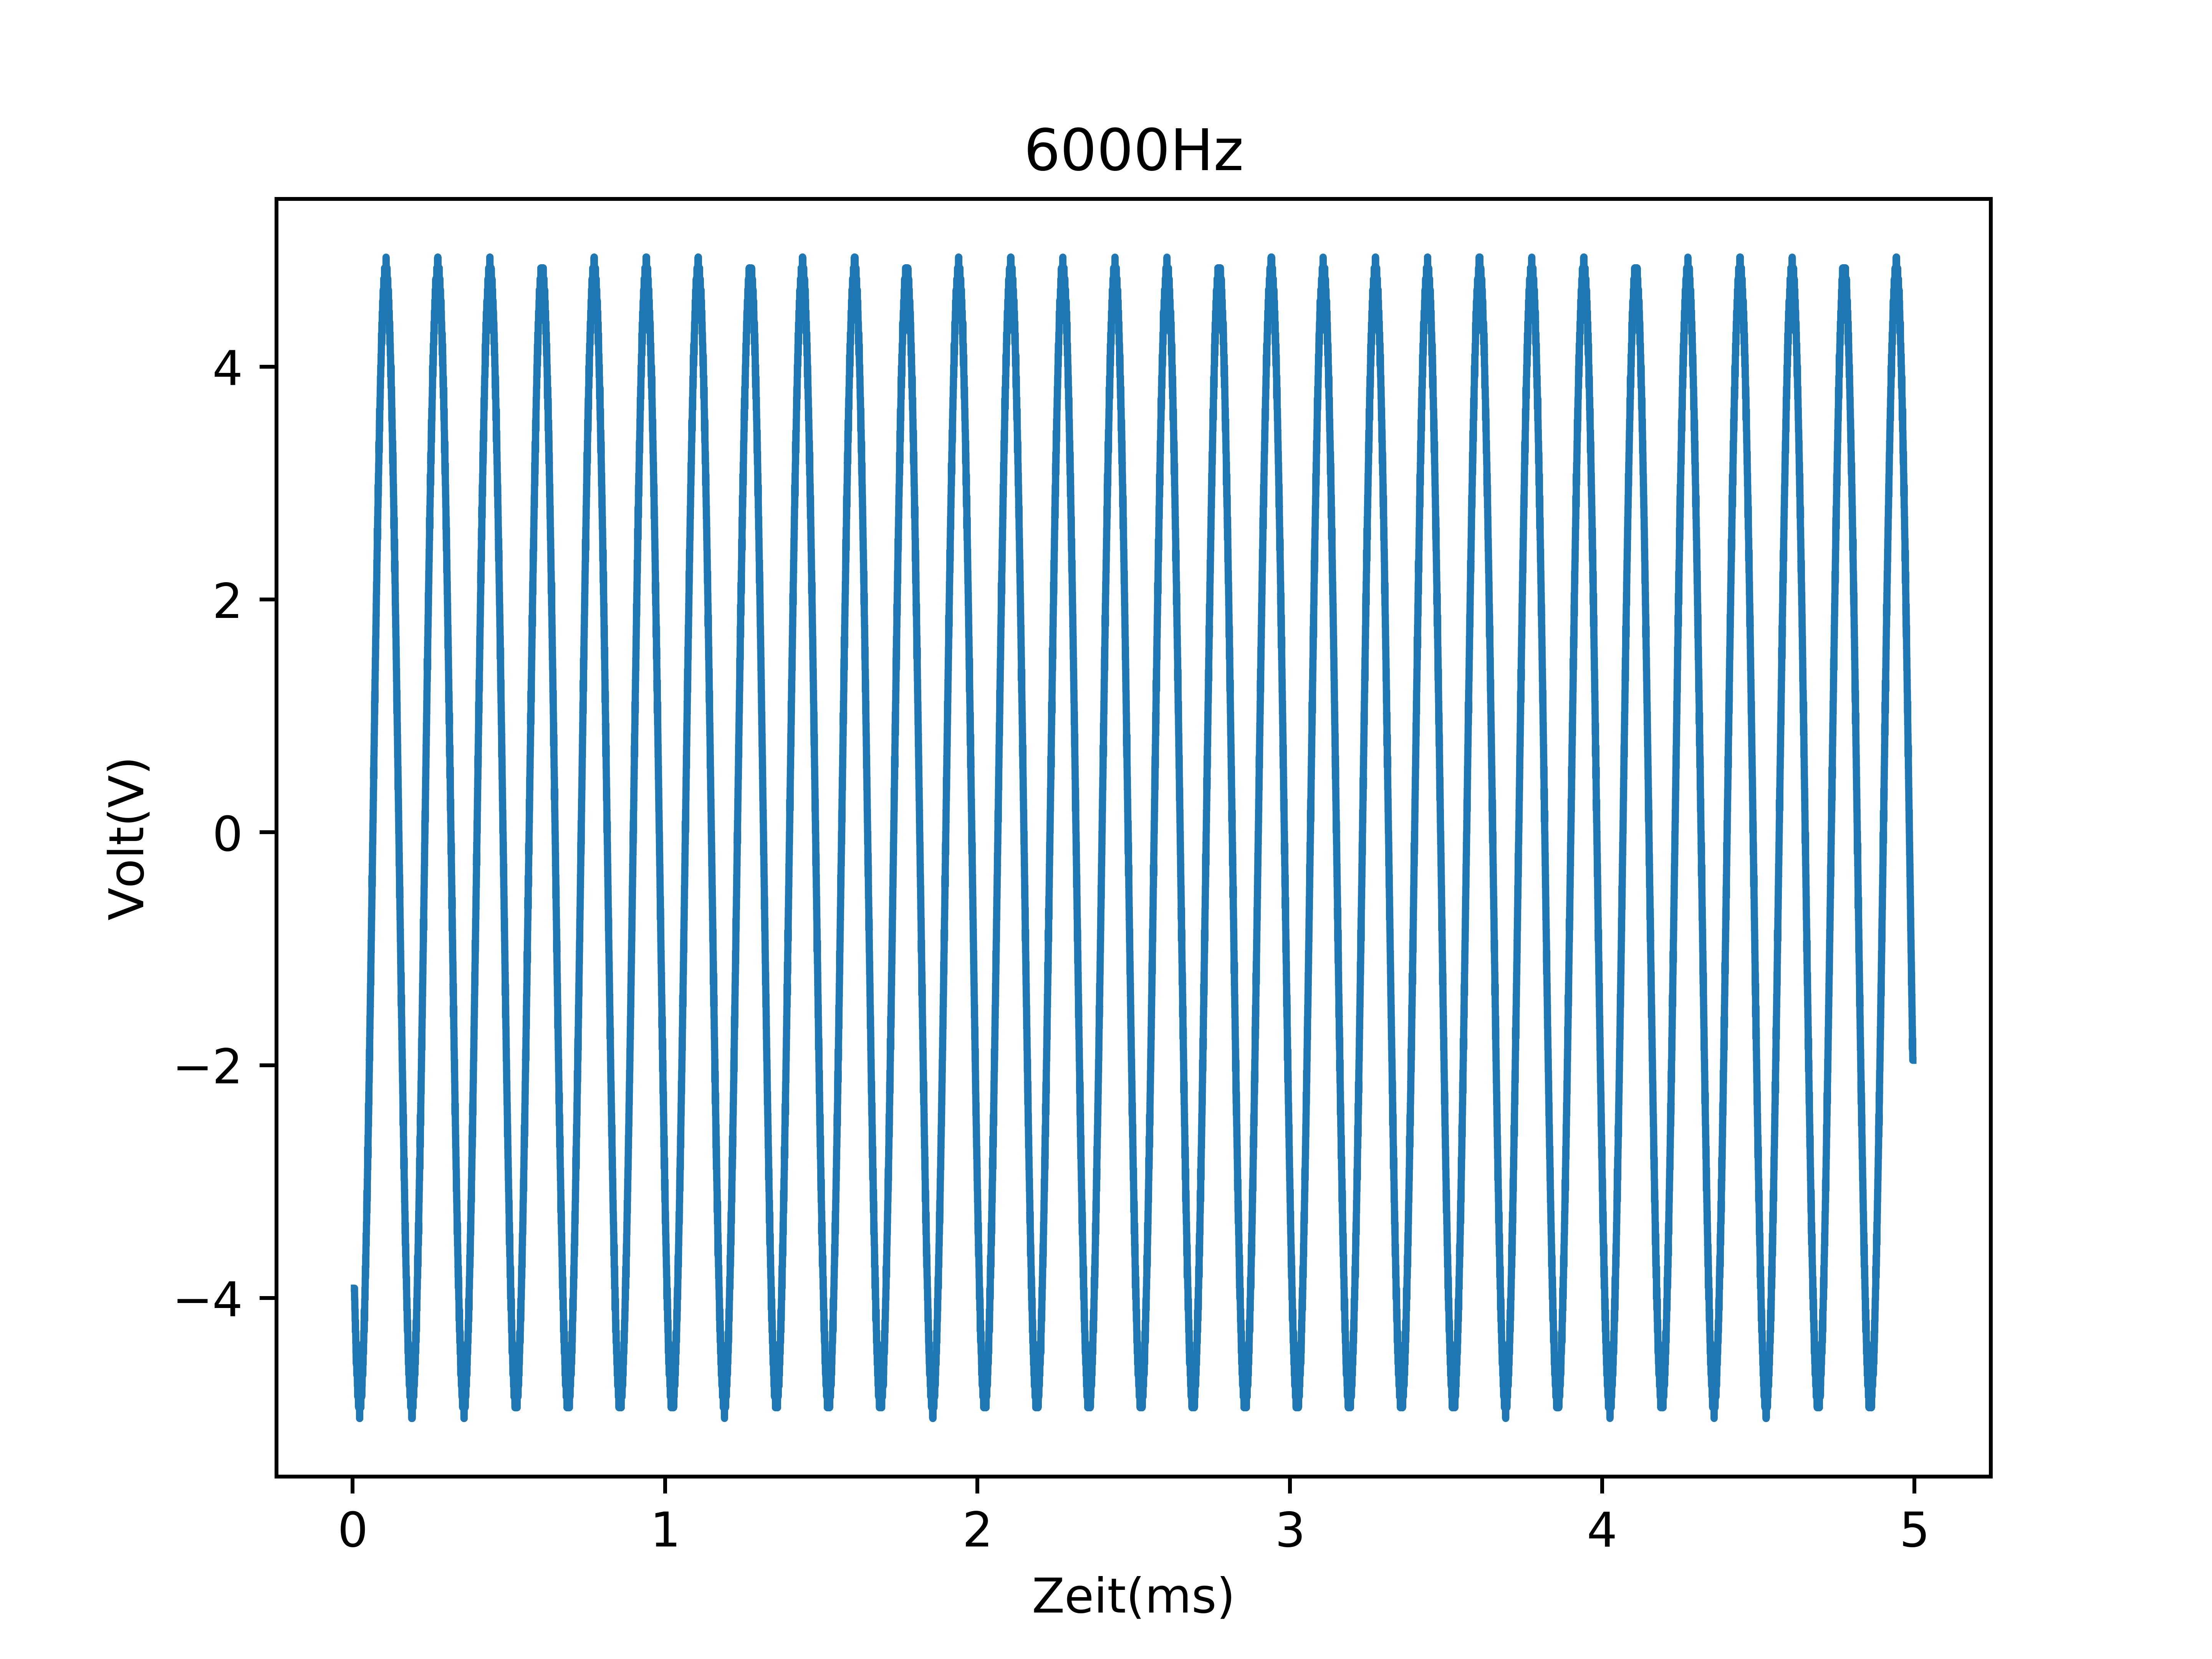
\includegraphics[width=0.8\textwidth]{../Images/6000Hz.png}
	\caption{6000Hz}
\end{figure}
\begin{figure}[H]
	\centering
	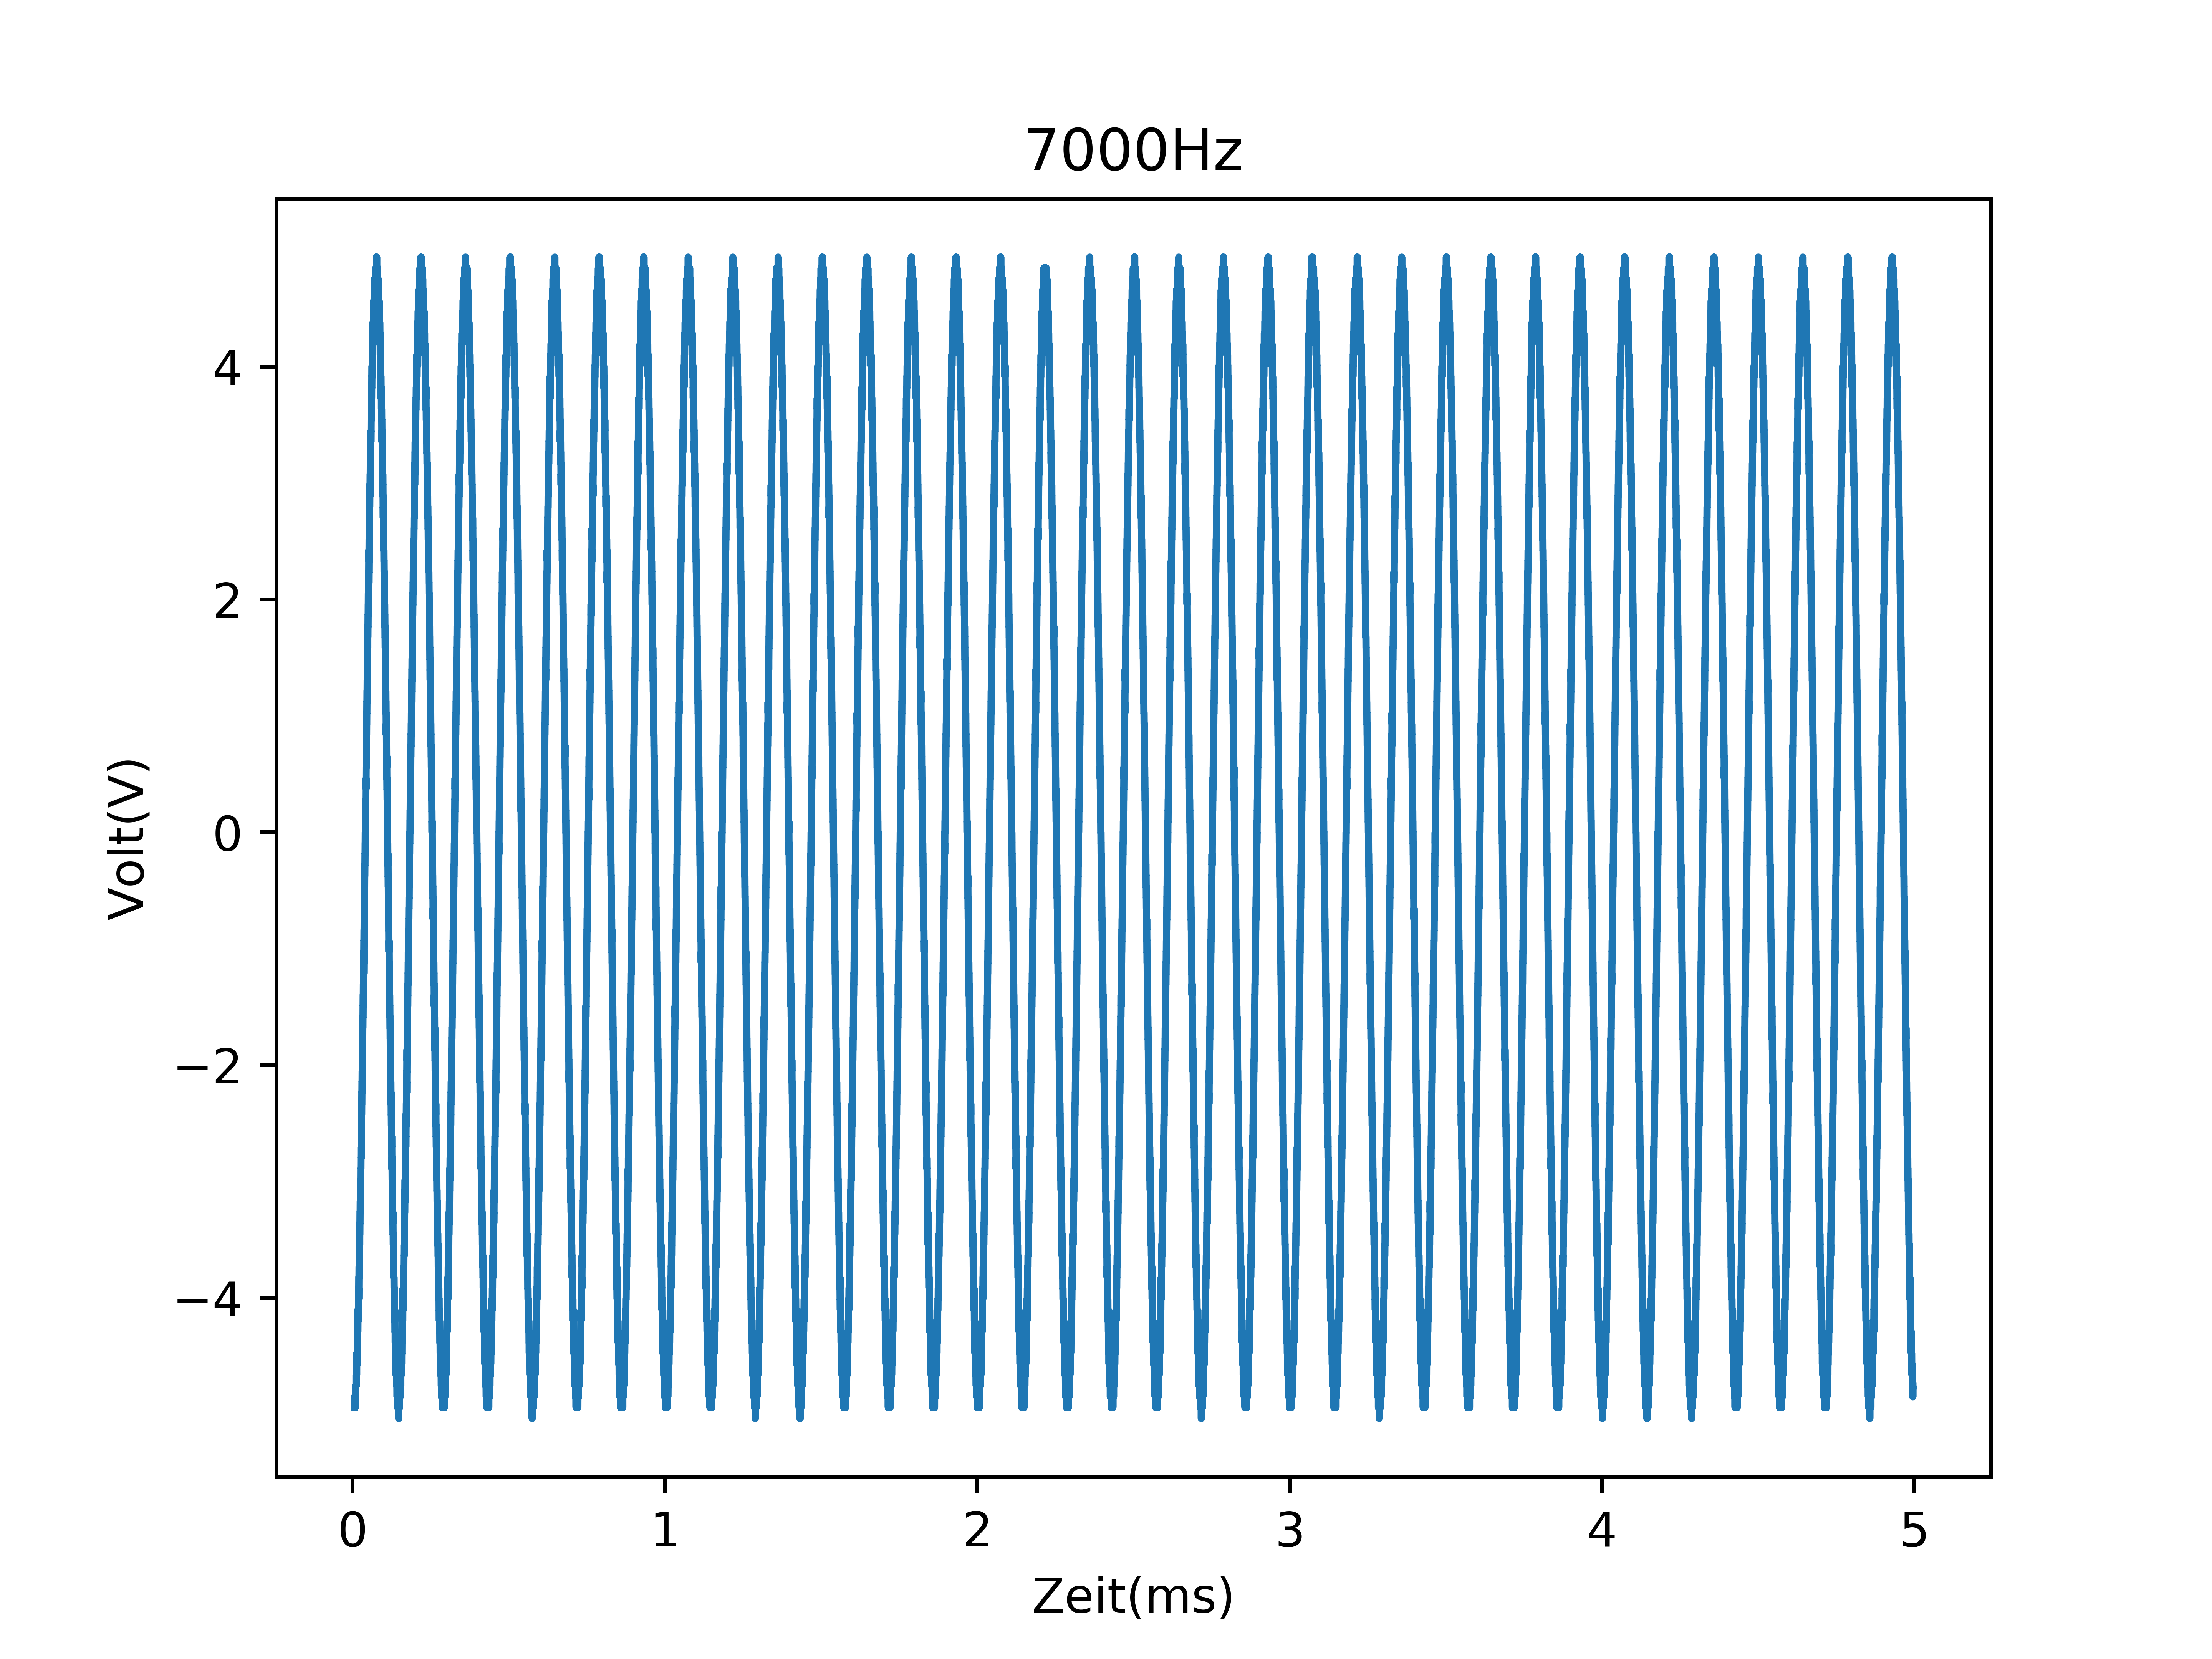
\includegraphics[width=0.8\textwidth]{../Images/7000Hz.png}
	\caption{7000Hz}
\end{figure}

\section{Interpretation}
\label{chap:VERSUCH_5_INTERPRETATION}
\begin{normalsize}
Wie im Code zu sehen ist haben wir 8000 als Samplingfrequenz angegeben. Ausgelesen haben wir jedoch 8021(Siehe Abbildung 6.1) welche der AD-Wandler als eigentlich Samplingfrequenz verwendet.
Die Nyquistfrequenz ist die hälfte der Samplefrequent welche in unserem Fall 8021 ist. Dadurch beträgt die Nyquistfrequenz also 8021 / 2 = 4010,5
\end{normalsize}
%
% CHAPTER Anhang
%
\renewcommand\thesection{A.\arabic{section}}
\renewcommand\thesubsection{\thesection.\arabic{subsection}}

\chapter*{Anhang}
\label{chap:APPENDIX}
\addcontentsline{toc}{chapter}{Anhang}
\setcounter{chapter}{0}
\addtocounter{chapter}{1}
\setcounter{section}{0}

\section{Quellcode}
\label{chap:APPENDIX_SOURCECODE}

\subsection{Quellcode Versuch 1}
\label{chap:APPENDIX_SOURCECODE_V1}
\lstinputlisting[style=PYTHON, frame=single, captionpos=b, caption=Code von Versuch 1 zum Auslesen von der Karte]{../Python/GetVoltage.py}
\pagebreak
\lstinputlisting[style=PYTHON, frame=single, captionpos=b, caption=Code von Versuch 1 zum Schreiben auf die Karte]{../Python/SetVoltage.py}
\pagebreak

\subsection{Quellcode Versuch 3}
\label{chap:APPENDIX_SOURCECODE_V3}
\begin{normalsize}
Siehe Quellcode von Versuch 1
\end{normalsize}
\pagebreak

\subsection{Quellcode Versuch 4}
\label{chap:APPENDIX_SOURCECODE_V4}
\lstinputlisting[style=PYTHON, frame=single, captionpos=b, caption=Code von Versuch 4 zum Erzeugen des Sinus]{../Python/Sinus.py}
\pagebreak

\subsection{Quellcode Versuch 5}
\label{chap:APPENDIX_SOURCECODE_V5}
\lstinputlisting[style=PYTHON, frame=single, captionpos=b, caption=Code von Versuch 5 zum Erzeugen der Graphen]{../Python/PlotGraphs.py}
\lstinputlisting[style=PYTHON, frame=single, captionpos=b, caption=Code von Versuch 5 zum Auslesen der Abtasfrequenz]{../Python/task5.py}

%
% Literaturverzeichnis
%
%
% Literaturverzeichnis
%
\phantomsection
\addcontentsline{toc}{chapter}{Literaturverzeichnis}
\bibliography{references}
\newpage

\end{document}
%------------------------------------
% ╔═╗╔╗╔╔╦╗  ╔╦╗╔═╗╔═╗╦ ╦╔╦╗╔═╗╔╗╔╔╦╗
% ║╣ ║║║ ║║   ║║║ ║║  ║ ║║║║║╣ ║║║ ║ 
% ╚═╝╝╚╝═╩╝  ═╩╝╚═╝╚═╝╚═╝╩ ╩╚═╝╝╚╝ ╩ 
%------------------------------------